\chapter{Implementation}
\label{chapter:implementation}
% \epigraph{The best presents don't come in boxes.}{Bill Watterson}
% \epigraph{Typing is no substitute for thinking.}{Dartmouth Basic manual, 1964}

This chapter is divided into two halves which detail the implementation of a Truffle interpreter and extensions for parametric polymorphism.
The first half of this chapter will describe the methods used to transform TASTy to make it suitable for a Truffle interpreter, \textsc{TastyTruffle}, \textit{without} polymorphism.
In particular, the first section covers how to translate the organization of data and code in the \scalainline{DefDef}, \scalainline{ClassDef}, and \scalainline{Term} tree nodes into a Truffle implementation which is amenable to execution and JIT optimization.
The second half of this chapter will then discuss extensions to our implementation support parametric polymorphism and cover the techniques we use to specialize nodes to eliminate autoboxing in the presence of polymorphism. 

\section{The Monomorphic Interpreter}
\label{impl:section:monomorphic}

Scala programs in \acrshort{tasty} format are unsuitable for execution in a Truffle interpreter. 
Programs in TASTy must be parsed and transformed into an executable representation in Truffle.
This involves translating the TASTy tree structure into a simpler, but semantically equivalent Truffle AST.
For the rest of this thesis, we refer to the Truffle AST of TASTy as \textit{TastyTruffle IR}.
As TASTy represents a Scala program close to its equivalent source representation, canonicalization compiler passes (see appendix \ref{appendix:dotty-phases}) that would otherwise normalize the IR are not present. 
Instead, we implement TastyTruffle IR to represent a canonicalized executable intermediate representation which can later be specialized on demand. 

\begin{figure}[!htb]
	\begin{minted}{scala}
	def evaluate(tree: Tree): Object = tree match {
		case vdef: ValDef   => 
			lazy val obj = initializeObject(vdef)
			registerObject(vdef.symbol, obj)			
		case cdef: ClassDef => 
			registerShape(cdef.tpe, parseClassDef(cdef))	
		case _ => ()
	}
	\end{minted}
	\caption{Pseudocode to evaluate every top level tree.}
	\label{impl:top-level}
\end{figure}

Figure \ref{impl:top-level} gives an evaluation loop that is common in other interpreters in the context of this one.
A top level tree is any tree without a parent.
In our subset of TASTy, a top level tree may be a \scalainline{ValDef} (a singleton object) or a \scalainline{ClassDef}.
Here we only present the pseudocode sufficient to traverse a program in TASTy. 
Each top level definition is parsed and saved.
Note that we intentionally omit \textit{how} to execute the program.
Entry points in \scalainline{TASTy} are defined by a special method \scalainline{main}.
As multiple entry points may exist in a given program, we consider the selection of entry points an implementation-specific detail.
In the following sections, we will describe the individual types of TASTy nodes and why some are directly unsuitable for execution and how to simplify their semantics for execution.

\subsection{Converting the \texttt{DefDef} tree into a Truffle Root Node}
\label{impl:subsection:defdef}

In this section, we describe the conversion of \scalainline{DefDef} trees to \textit{root nodes}.
\scalainline{DefDef} trees are the primary structure which organizes code (terms) in TASTY.
Root nodes represent the root of an executable Truffle AST, the primary abstraction which organizes code in Truffle.
In our case, root nodes are the Truffle analog of a \scalainline{DefDef}.
Each root node has a corresponding \textit{call target}, which is used for invocation of the root node.
Call targets are the primary compilation unit for Graal.
A compilation unit is an organization of code which can be independently compiled.
A root node is automatically instrumented\cite{profiling:atom} to profile its number of invocations. 
When a root node has been frequently invoked inside the interpreter, it is JIT compiled into machine code by Graal.
Subsequent invocations of the call target will then use the more efficient compiled root node.

\begin{figure}[!htb]
	\begin{minted}{scala}
	abstract class RootNode(desc: FrameDescriptor) {
		def execute(frame: VirtualFrame): Object
		def getCallTarget: CallTarget
	}
	\end{minted}
	\caption{Pseudocode of a root node.}
	\label{example:root-node}
\end{figure}

Figure \ref{example:root-node} gives a simplified implementation of a root node.
Each root node in Truffle has a \textit{frame descriptor} and execution semantics.
A guest language must subclass and implement its own root node in order to enable function invocation semantics.

A frame descriptor describes guest language variables which are in scope during execution.
The abstract \javainline{execute} method describes the invocation behaviour of a root node.
When a root node is executed, it always supplied with a \textit{frame}.
A frame contains the arguments supplied during invocation and storage slots for local variable definitions in the body of the method.
By default, all frames start off \textit{virtual}.
Virtual frames are Truffle abstractions that provide guest languages an opportunity to exploit escape analysis.
Escape analysis\cite{escape-analysis} reasons about the dynamic scope of object allocations. 
Truffle and Graal both exploit the observations of \textit{Partial Escape Analysis}\cite{java:partial-escape-analysis}, a path-sensitive variant of escape analysis, to enable the following optimizations for guest languages:

\begin{description}
	\item[Region Allocation\cite{java:escape-analysis}\cite{tofte:region-memory}] The substitution of heap allocations with stack allocations to eliminate unnecessary garbage collection.
	\item[Scalar Replacement\cite{java:escape-analysis-optimizations}] The complete elimination of an object allocation, where the fields of the replaced object are substituted by local variables.
\end{description}

The virtual frame abstraction allows guest languages to read and write to a frame without the requirement to optimize their object allocations.
Instead, escape analysis and subsequently scalar replacement is responsible for optimizing guest language object allocations during partial evaluation. 

\begin{figure}[!htb]
	\begin{minted}{scala}
	class DefDef(_: String, params: List[ParamClause], _: TypeTree, rhs: Option[Term]) extends Definition	
	\end{minted}
	\caption{Defintion of a \texttt{DefDef} tree with names of less important members replaced with \texttt{\_}}
	\label{recall:defdef}
\end{figure}

A further simplified definition of a \scalainline{DefDef} tree is provided in figure \ref{recall:defdef}.
In this section, we focus on two members of a \scalainline{DefDef} trees.
The parameters of a \scalainline{DefDef} tree are given by the \scalainline{params} field.
In practice, the type of a \scalainline{ParamClause} is an alias for the union type \scalainline{TypeParams {|} TermParams}, so we omit the \scalainline{ParamClause} definition.
A \scalainline{DefDef} tree will have a parameter section for type parameters when they are polymorphic and will always have term parameters section.
\scalainline{DefDef} trees may optionally have a body defined in the \scalainline{rhs} field.
When trees do not have a body defined, they are abstract method definitions and do not have  corresponding root node in Truffle.
We will only consider non-abstract method definitions which have a body (a term) defined to be executable.
We will cover the parsing of terms into nodes for execution in detail after section \ref{impl:subsection:classdef}

\begin{figure}[!htb]
	\begin{minted}{scala}
	object FrameSlotKind extends Enumeration {
		type FrameSlotKind = Value
		val Object, Long, Int, Double, Float, Boolean, Byte = Value
	}	
		
	def getFrameSlotKind(tpe: Type): FrameSlotKind = 
		if (tpe.isPrimitive) 
			getPrimitiveSlotKind(tpe) // Int => FrameSlotKind.Int, ..., Double => FrameSlotKind.Double
		else  
			FrameSlotKind.Object
	\end{minted}
	\caption{Simplified implementation of \scalainline{FrameSlotKind}}
	\label{impl:frameslot-kind}
\end{figure}

Each value definition in the parameters of a \scalainline{DefDef} will have a corresponding frame slot in its parent frame descriptor. 
A frame slot references a unique frame value in the context of a root node.
Truffle permits each frame slot in a frame descriptor be described by a \textit{frame slot kind}.
In Truffle, there is a corresponding frame slot kind for reference types and each \acrshort{jvm} primitive type. 
Pseudocode of a frame slot kind and a method to convert a type into a slot kind is given in \ref{impl:frameslot-kind}.

Truffle profiles frame accesses in order to minimize the amount of autoboxing which occurs when reading from frame slot with an \javainline{Object} kind. 
To eliminate unnecessary specialization of frame accesses where types are monomorphic and statically refer to a primitive type, a parameter is assigned the matching primitive frame slot kind in the frame descriptor. 
In cases where the type is not a primitive type or a polymorphic applied type, e.g. \scalainline{List[T]} but not \scalainline{T}, we assign its frame slot the \scalainline{Object} kind.
Otherwise, the type is a polymorphic parameter which \textit{could} resolve to a primitive type and the frame slot kind cannot be resolved statically.
We will defer discussion on how to handle parameters of such polymorphic types that cannot be resolved statically until section \ref{implementation:specialization}.

\begin{figure}[!htb]
	\begin{minted}{scala}
	case class LocalVal(slot: FrameSlot, kind: FrameSlotKind)
		
	class DefDefNode(desc: FrameDescriptor, params: Array[LocalVal], body: TermNode) extends RootNode(desc) {
		override def execute(frame: VirtualFrame): Object = {
			copyArgumentsToFrame(frame)
			try {
				body.execute()
			} catch {
				case ex: ReturnException => ex.getValue
			}
		}	
			
		def copyArgumentsToFrame(frame: VirtualFrame): Unit = 
			for ((param, arg) <- params zip frame.getArguments) 
				param.kind match {
					case FrameSlotKind.Int =>
						frame.setInt(param.slot, arg.asInstanceOf[Int])
					...
					case FrameSlotKind.Double =>
						frame.setDouble(param.slot, arg.asInstanceOf[Double])	
					case _ =>
						frame.setObject(param.slot, arg)
				}
	}
	\end{minted}
	\caption{Pseudocode for \scalainline{DefDefNode} and \scalainline{Parameter}}
	\label{impl:defdefnode}
\end{figure}

Figure \ref{impl:defdefnode} provides the implementation of the \scalainline{DefDefNode} and its parameters, the root node equivalent of a \scalainline{DefDef}.
The execution of a \scalainline{DefDefNode} is divided into two stages, argument preparation and execution.
First, the arguments of the frame constructed during invocation (see \ref{impl:subsection:apply}), are copied into their respective parameter frame slots.
Frames contains separate regions for values of each frame slot kind.
Based on the frame slot kind prescribed to a parameter, we copy each argument into the appropriate frame slot region.
Storing parameters in this manner eliminates any unnecessary unboxing which would otherwise occur during a frame access.
After arguments are copied into the frame, their values become available for access during the execution of the body.
The body of a \scalainline{DefDefNode} is then executed and its computed value returned.

\begin{figure}[!htb]
	\begin{minted}{scala}
	def parseDefDef(ddef: DefDef): DefDefNode = {
		val desc = new FrameDescriptor
		val parameters = self :: ddef.params.map {
			case vdef: ValDef => createParameter(vdef, desc)
		}
			
		val body = parse(ddef.rhs)
		new DefDefNode(desc, parameters, body)
	}
		
	def createParameter(vdef: ValDef, desc: FrameDescriptor): LocalVal = {
		val kind = getFrameSlotKind(vdef.tpt.tpe)
		val slot = desc.addSlot(kind)
		Parameter(slot, kind)
	}
	\end{minted}
	\caption{Pseudocode for parsing \scalainline{DefDef} into \scalainline{DefDefNode}}
	\label{impl:parse-defdef}
\end{figure}

Figure \ref{impl:parse-defdef} provides a summary on parsing a \scalainline{DefDef} tree into its Truffle equivalent \scalainline{DefDefNode}.
Frame slot and a frame slot kinds provide an abstraction for parameters and arguments to be resolved before the execution of the main body in a \scalainline{DefDefNode}.
In addition to the parameters which are explictly present in TASTY, the root node will have additional parameter which represents the receiver of the method.
The receiver is an object instance whose class definition owns the method being invoked.
In Scala, every method invocation has a receiver.
In TASTy, this translates to every \scalainline{DefDef} is owned by a \scalainline{ClassDef}.
In the next section, we detail how to organize call targets in Truffle by using \scalainline{ClassDef} trees.

\subsection{Deriving Shapes from \texttt{ClassDef} trees}

\begin{figure}[!htb]
	\centering
	\begin{subfigure}[b]{0.48\textwidth}
	\begin{minted}{scala}
	class ClassDef(
		name:        String,
		constructor: DefDef, 
		parents:     List[Tree], 
		_:           Option[ValDef], 
		body:        List[Statement]
	) extends Definition
		\end{minted}
	\caption{Pseudocode of a \scalainline{ClassDef}.}
	\label{recall:classdef}
	\end{subfigure}
	\hfill
	\begin{subfigure}[b]{0.48\textwidth}
	\begin{minted}{scala}
	class ClassShape(
		symbol:  Symbol,
		parents: Array[Symbol],
		fields:  Array[Field]
		methods: Map[MethodSignature, CallTarget]
		vtable:  Map[MethodSignature, Symbol]
	)
	\end{minted}
	\caption{Pseudocode of a shape for a \scalainline{ClassDef}.}
	\label{impl:classshape}
	\end{subfigure}
\end{figure}

\scalainline{ClassDef} tree define the layout of an object in TASTy.
The layout of a object dictate the values which an object instance stores as well the methods which can be invoked on an object instance.
The data layout of an object in a Truffle interpreter is described by a \textit{shape}\cite{self:prototypes}\cite{truffle:object-model}.
Shapes are a language-agnostic model for defining the properties of a object instance in Truffle.
A property in a shape describes one member of an object instance; it has an identifier and a value.
A Truffle object instance consists of \textit{object storage}, which contains instance-specific data, and its shape.
Shapes map property identifiers to object storage locations; guest languages interface with object storage indirectly through properties.
In this thesis we use a \textit{static shape}, an immutable variant of a shape.
Normally, shapes are mutable and their list of properties may change throughout the lifetime of a program\cite{truffleruby:object-model}.
However, programs which dynamically change the layout of their objects\cite{java:reflection} are out of the scope of this thesis.

\begin{figure}[!htb]
	\begin{minted}{scala}
	def parseClassDef(cdef: ClassDef): ClassShape = {
		val parents = cdef.parents.map(_.symbol)
		
		val fields = cdef.body map {
			case vdef: ValDef => generateField(vdef)	
		}
		
		val methods = (cdef.constructor :: cdef.body) map {
			case ddef: DefDef => ddef.symbol.signature -> parseDefDef(ddef)
		}
		
		val vtable = cdef.symbol.methodMembers map {
			symbol => symbol.signature -> symbol
		}
	
		new ClassShape(cdef.symbol, parents, fields, init ++ methods, vtable)
	}

	def generateField(vdef: ValDef): Field = vdef match {
		case ValDef(_: String, tpt: TypeTree, rhs: Option[Term]) => new Field(vdef.symbol, )
	}
	\end{minted}
	\caption{Pseudocode to convert a \scalainline{ClassDef} into a \scalainline{ClassShape}.}
	\label{impl:parse-classdef}
\end{figure}

Recall the definition of a \scalainline{ClassDef} in figure \ref{recall:classdef}.
Each \scalainline{ClassDef} tree can be parsed into a corresponding \scalainline{ClassShape}, given in Figure \ref{impl:classshape}.
Figure \ref{impl:parse-classdef} provides a very simplified implementation of the parsing steps to transform a \scalainline{ClassDef} into a \scalainline{ClassShape}.
The \scalainline{name} parameter of \scalainline{ClassDef} alone is insufficient to be used as an identifier for a \scalainline{ClassShape}.
Names do not disambiguate between classes of the same name declared in different packages.
Instead, we used the symbol of the \scalainline{ClassDef} tree as the identifier for the \scalainline{ClassShape}.
For the remainder of this thesis, we will use a \scalainline{ClassInstance} to refer to an object instance with properties described by a \scalainline{ClassShape}.

\begin{figure}[!htb]
	\begin{minted}{scala}
	class Field(symbol: Symbol, tpe: Type) extends StaticProperty {
		override def getId: String = symbol.name
			
		def get(instance: Object): Any = 
			if (tpe == Int) getInt(instance)
			else if ...
			else if (tpe == Double) getDouble(instance)
			else getObject(instance)
	
			
		def set(instance: Object, value: Any): Unit = 
			if (tpe == Int) setInt(instance, value.asInstanceOf[Int])
			else if ...
			else if (tpe == Double) setDouble(instance, value.asInstanceOf[Double])
			else setObject(instance, value)	
	} 
	\end{minted}
	\caption{Pseudocode of the field property.}
	\label{impl:field}
\end{figure}

A \scalainline{ValDef} tree in the body of a \scalainline{ClassDef} translates to a field definition in the \scalainline{ClassShape}.
A \scalainline{ClassShape} has an collection of fields, which implement the static shape property.
Figure \ref{impl:field} gives our implementation of a field.
Fields define operations to read and write from the object storage on a \scalainline{ClassInstance}.
Like frames with frame slot kinds, object instances in Truffle have separate regions for storing values of each primitive type and one for reference types.
Following the same rules with types and frame slot kinds described in section \ref{impl:subsection:defdef}, the data access of a field depends on the type of the \scalainline{ValDef} tree from which the field originates.
The remaining members of a \scalainline{ClassShape} do not describe data which has to be stored in the object storage of a \scalainline{ClassInstance}.

\begin{figure}[!htb]
	\begin{minted}{scala}
	case class MethodSignature(symbol: Symbol, params: Int, types: Array[Type])
	\end{minted}
	\caption{Pseudocode of a method signature.}
	\label{impl:method-signature}
\end{figure}

After the constructor and the \scalainline{DefDef} statements of a \scalainline{ClassDef} are converted into root nodes, they are stored in the \scalainline{ClassShape} mapped by a method signature.
The pseudocode for a method signature is given in figure \ref{impl:method-signature}.
Method signatures disambiguate method invocations in the presence of \textit{ad hoc polymorphism}\cite{strachey:fundamental-concepts}, where methods share the same name but have different arguments.
When combined with parametric polymorphism, method signatures must also be able to disamibguate between methods sharing the same name but having different type parameters.
However, method signatures do not have to disambiguate between different type parameters by name, only the number of type parameters that a method has.
Because type erasure erases polymorphic type parameters from methods, methods which share the same number of parameters as well as the same arguments will conflict and therefore are invalid.
As previously mentioned, methods are shared between all \scalainline{ClassInstance} objects with the same shape, call targets are stored on the shape itself.

Often a shape will not contain the call target referenced by a signature because the dispatch is dynamic and the original type inherits the method.
A \scalainline{ClassShape} contains a \textit{virtual method table}, which maps a method signature to the symbol of a shape which contains the call target matching the signature.
If a method signature does not have a call target in the current shape, the shape which holds the target is indirectly resolved using the virtual method table during execution.
While this resolution carries signficant performance overhead both in Truffle and other implementations of programming languages, we will describe a technique which partially mitigates this overhead further on this half of chapter.

\subsection{Transforming \texttt{Terms} into \texttt{Nodes}}

\begin{figure}[!htb]
	\begin{minted}{scala}
	abstract class TermNode extends Node with InstrumentableNode {
	
		def execute(frame: VirtualFrame): Object 
		def executeInt(frame: VirtualFrame): Int = execute(frame).asInstanceOf[Int]
		...
		def executeDouble(frame: VirtualFrame): Double = execute(frame).asInstanceOf[Double]

	}
	\end{minted}
	\caption{Pseudocode of a TermNode.}
	\label{impl:term-node}
\end{figure}

In this section we will cover the conversion of a \scalainline{Term} trees into Truffle nodes.
The Truffle \scalainline{Node} abstraction allows guest languages to implement executable fragments of an AST.
Figure \ref{impl:term-node} is our subclass of a Truffle \scalainline{Node}.
Subclasses of the \scalainline{TermNode} will define node-specific semantics encapsulating a particular functionality of the interpreter.
The \scalainline{TermNode} takes advantage of Truffle's autoboxing elimination by defining companion \scalainline{execute[TYPE]} methods to allow subclasses to declare when an expected result from a child node must conform to a specific primitive type.
In the following subsections, we give the subclasses which individually implement functionality of the monomorphic interpreter.

\subsubsection*{Creating Instances}

\begin{figure}[!htb]
	\begin{minted}{scala}
	def parseNew(new: New): NewNode = new NewNode(new.tpe.symbol)	
	
	class NewNode(symbol: Symbol) extends TermNode {
		override def execute(frame: VirtualFrame): Object =  shapeOf(symbol.tpe).newInstance
	}
	\end{minted}
	\caption{Pseudocode of a \scalainline{NewNode} and how it is parsed.}
	\label{impl:new-node}
\end{figure}

The \scalainline{New} tree represents the allocation of an instance of a \scalainline{ClassDef}.
The Truffle equivalent allocate node given in figure \ref{impl:new-node} is not so different, but it allocates an instance with properties described by the \scalainline{ClassShape} instead of a \scalainline{ClassDef}.
Note that a \scalainline{NewNode} only \textit{creates} an object; the parameters and fields of an object remain uninitialized.
An object is \textit{initialized} when the initializer, \scalainline{<init>}, method is invoked on a newly created object.
TASTy is emitted with this sequence of events in mind, object creation is always followed by object initialization.
Structurally, this means that a \scalainline{New} tree is always the child of an initializer \scalainline{Apply} tree.

\subsubsection*{Function Application}
\label{impl:subsection:apply}

\begin{figure}[!htb]
	\begin{minted}{scala}
	def parseApply(apply: Apply): ApplyNode = {
		val signature = apply.symbol.signature
		apply match {
			case Apply(Select(qualfier, _), arguments) => 
				if (qualifier.tpe.isPrimitve)
					if (args.length == 0) unaryOp(signature, qualifier)
					else                  binaryOp(signature, qualifier, args(0))
				else if (qualifier.tpe.isArray)
					arrayOp(signature, qualifier, arguments)
				else 
					new ApplyNode(signature, parse(qualifier), arguments.map(parse))	
			}
		}
	\end{minted}
	\caption{Pseudocode of parsing an \scalainline{Apply} tree.}
	\label{impl:parse-apply}
\end{figure}
The \scalainline{Apply} tree is a context-dependent tree which represents multiple types of operations.
These operations are disambiguated by the types of their receiver.
Figure \ref{impl:parse-apply} provides an overview on the transformations discussed in this section as pseudocode for parsing an \scalainline{Apply} into TastyTruffle IR.
We omit the implementations of \scalainline{unaryOp}, \scalainline{binaryOp}, \scalainline{arrayOp} to remain concise; 
These methods generate an Truffle intrinsic node intrinsic which represent a similar JVM equivalent.
In the following subsections, we enumerate all possible semantics in our subset of TASTy:

\paragraph{Arithmetic and Logical Operators}

In TASTy there are no unary and binary operators typically found in Java or other imperative languages.
Unary and binary operators are actually an invocation of 0-argument (unary operator) or 1-argument (binary operator) method. 
For example, the following addition operator in Scala \scalainline{1 + 2} is desugared to \scalainline{1.+(2)}. 
That is, the binary operator \scalainline{+} is represented as the invocation of the instance function \scalainline{Int.+} on the receiver with value \scalainline{1} and type \scalainline{Int} with a single argument \scalainline{2}.
Normally in the Scala compilation pipeline, methods which operate on primitive types and have an equivalent bytecode instruction on the JVM\cite{java:vm-spec} are replaced by those instructions in compiled program bytecode. 
This process of selecting efficient implementations for numerical or logical operations is commonly known as intrinsification.
Similarly, TastyTruffle avoids implementing methods of primitive types with actual call semantics as primitive operations are frequently used and simplify optimization for Graal.

\paragraph{Array Access}

The syntax for accessing array elements in Scala does not differ from the invocation of method on an array.
In other imperative languages such as Java, the syntax for accessing arrays is commonly separate from the syntax of invoking a method.
For example, the access \scalainline{array(0)} is desugared to \scalainline{array.apply(0)} once the program is emitted in TASTy.

Similar to unary and binary operators, the underlying implementation of array operations are intrinsified into JVM bytecode instructions where possible.
However, using the bytecode provided in figure \ref{example:contains-bytecode} as an analog, operations on polymorphic arrays \scalainline{cannot} be intrinsified.
Instead, polymorphic array operations are handled by functions in the Scala runtime library.
The overhead of such operations are substantial and commonly represent the largest performance bottlenecks in array-bound programs.
These costs are additionally abstracted from the user as they commonly arise when using array-backed collections from the Scala standard library.

To operate without specialization, the implementation of our interpreter also incorporates the same runtime code to handle polymorphic array operations.
In the second half of this chapter, we will discuss the methods used to eliminate the runtime overhead of these polymorphic bridge methods.

\paragraph{Method Invocation}

\begin{figure}[!htb]
	\begin{minted}{scala}
	@NodeChild("receiver")
	@NodeField("signature", MethodSignature.class)
	class ApplyNode(@Children args: Array[TermNode]) extends TermNode {
		final val INLINE_CACHE_SIZE: Int = 5;
		
		@Specialization(guards = "instance.getShape == shape", limit = "INLINE_CACHE_SIZE")
		def cached(
			frame: VirtualFrame,
			instance: ClassInstance,
			@Cached("instance.getShape") shape: ClassShape,
			@Cached("create(resolveCall(instance, signature)") callNode: DirectCallNode
		): Object = callNode.call(evalArgs(frame, instance));
		
		@Specialization(replaces = "cached")
		def virtual(
			frame: VirtualFrame,
			instance: ClassInstance,
			@Cached callNode: IndirectCallNode
		): Object = {
			val callTarget = resolveCall(instance.getShape, signature);
			callNode.call(callTarget, evalArgs(frame, instance))
		}
	}
	\end{minted}
	\caption{Simplified implementation of the call node with a polymorphic inline cache used in TastyTruffle.}
	\label{implementation:poly-cache-call-node}
\end{figure}

Otherwise, the \scalainline{Apply} tree actually encodes a `normal' method invocation.
Truffle provides two abstractions for call nodes, the \textit{direct call node} is used when the call target can be statically resolved. 
In our subset of TASTy, this is the set of methods which have private or final modifiers\cite{java:lang-spec} and class constructors. 
Otherwise, the Truffle \textit{indirect call node} is used for calls where call targets must be dynamically resolved. 
Using indirect calls instead of direct calls comes with performance overhead as indirect call nodes cannot be inlined and inhibits Graal's dynamic intraprocedural analyses.
In this thesis, we describe a singular call node implementation for both statically and dynamically dispatched calls. 
In order to minimize the use of indirect call nodes, we take advantage of a polymorphic inline cache\cite{self:polymorphic-inline-caches} to eliminate the overhead of resolving virtual calls for \acrshort{jit} compilation. 

Figure \ref{implementation:poly-cache-call-node} shows a simplified Truffle call node in \textsc{TastyTruffle} which implements a polymorphic inline cache.
The \scalainline{ApplyNode} is declared using the Truffle DSL.
The \scalainline{@NodeChild} and \scalainline{@NodeField} annotations declare that the DSL should generate children and properties of those names and types respectively. 
The \scalainline{@Specialization} annotation declares the node writing semantics for method invocation.
Because we have defined a limit on the number of specializations, the DSL will also generate additional code for a polymorphic inline cache.
This cache saves call targets based on the type of receiver seen at the call site. 

When the type of receiver has not been seen in the inline cache, an additional cache entry is generated and appended to the cache for the next call.
Because a polymorphic inline cache dispatches direct calls based on the type of the receiver value seen, Graal is able to speculatively optimize the call site with the assumption that the receiver is always the same type and therefore the call target does change between invocations.
Furthermore, this allows the calls site to be inlined, allowing a feedback loop of intraprocedural optimizations\cite{conditional-constant-prop}\cite{variable-congruence} to propagate through the inlined tree.
One important aspect to note is the size of an polymorphic inline cache must be kept reasonable such that the cost of searching the cache should not defeat the speedup afforded by using the cache.
If the size of the cache exceeds the limit set, the call node is rewritten to use an indirect call as the cost of inline cache lookup will outweigh the penalty of an indirect call. 

\begin{figure}[!htb]
	\centering
	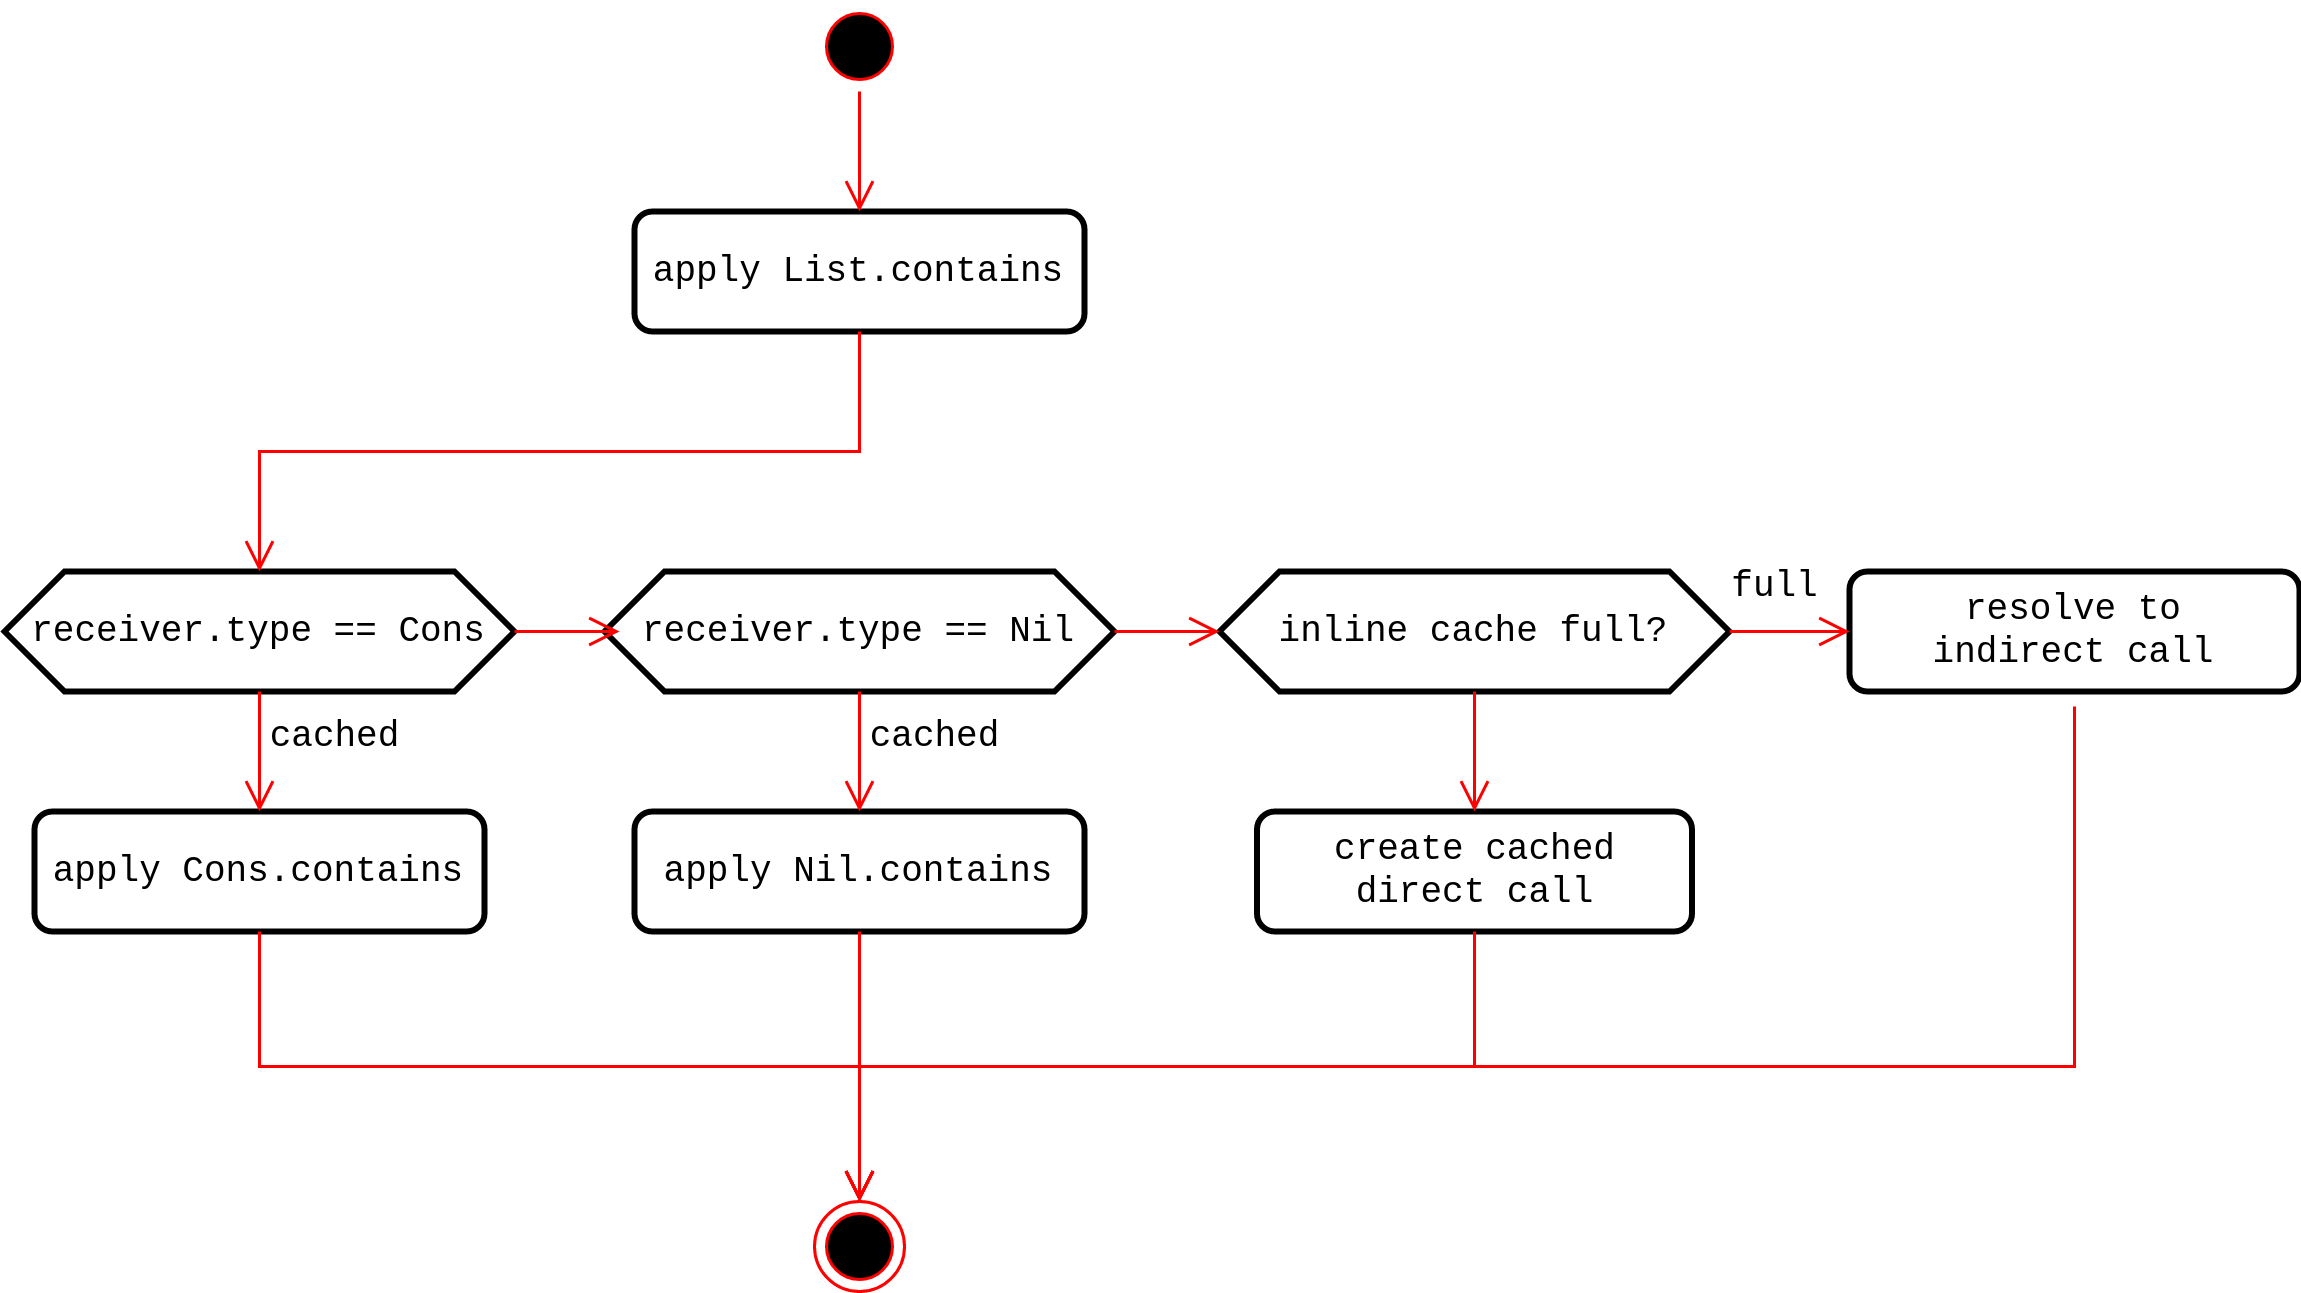
\includegraphics[width=0.6\textwidth]{figures/tastytruffle-pic-example.png}
	\caption{A possible polymorphic inline cache for a \scalainline{List.contains} callsite.}
	\label{example:poly-cache-call-node}
\end{figure}

Figure \ref{example:poly-cache-call-node} shows a data flow diagram of the application of a polymorphic inline cache to a call site of \scalainline{contains} when the receiver type is statically known to be \scalainline{List}. 
The diagram shown assumes that the call site has previously been called with a receiver where the dynamic type has been both \scalainline{Cons} and \scalainline{Nil}.
The \scalainline{ApplyNode} will first check if the type of receiver at the call site has the type \scalainline{Cons}; If the check passes then the cached direct call node is invoked and the call is complete.
It will then do the same for the type \scalainline{Nil}.
Otherwise, the type of the receiver has not been seen before and the call target is resolved virtually then cached for the next invocation at this call site.

When the polymorphic inline cache is applied to a monomorphic call site (where the type of the receiver does not change), it simplifies to a single element inline cache\cite{smalltalk:inline-caches}. 
Because the type of the receiver at the call site remains stable, the cache look up of the call target based on the type always succeeds and the call site never fallbacks to using an indirect call node.

\subsubsection*{Accessing Fields}

In our subset of TASTy, the \scalainline{Select} tree represents a read of a field of a \scalainline{ClassInstance}.
Notice in the resolution of the \scalainline{Apply} tree that an \scalainline{Apply} tree represents a method invocation when the applicator is a \scalainline{Select}.
Because functions are first-class objects in Scala, the TASTy tree for a method invocation is the access of a method as if it were a field then the application of the subsequent function value read to a list of arguments.
Since this case is handled previously when parsing the \scalainline{Apply} tree, a \scalainline{Select} tree always selects a value definition.

\begin{figure}[!htb]
	\begin{minted}{scala}
	@NodeChild("receiver")
	@NodeField("symbol", Symbol.class)
	abstract class ReadFieldNode extends TermNode {
		final val INLINE_CACHE_SIZE: Int = 3;
			
		@Specialization(guards = "instance.getShape == shape", limit = "INLINE_CACHE_SIZE")
		def cached(
			instance: ClassInstance,
			@Cached("instance.getShape") shape: ClassShape,
			@Cached("lookupField(shape)") field: Field
		): Object = field.getContents(instance)
			
		@Specialization(replaces = "cached")
		def virtual(instance: ClassInstance): Object = {
			val field = lookupField(instance.getShape)
			field.getContents(instance)
		}
	
		private def lookupField(shape: ClassShape): Field = shape.getField(symbol)
	}
	\end{minted}
	\caption{Pseudocode of field read node with a polymorphic inline cache.}
	\label{impl:field-read-node}
\end{figure}

Figure \ref{impl:field-read-node} gives a simplified implementation of a field read node.
Like the virtual dispatch of call targets, fields are resolved dynamically with the shape of a \scalainline{ClassInstance}.
We apply a polymorphic inline cache to the lookup of field properties to eliminate the performance overhead associated with this kind of virtual dispatch.

\subsubsection*{Accessing Locals and Globals}

\begin{figure}[!htb]
	\begin{minted}{scala}
	def parse(ident: Ident): TermNode = {
		if (ident.symbol.isObjectDef)
			new ReadGlobalNode(symbol)
		else 
			new ReadLocalNode(localOf(symbol))
	}
	\end{minted}
	\caption{Pseudocode to parse an \scalainline{Ident} tree.}
	\label{impl:parse-ident}
\end{figure}

The \scalainline{Ident} tree is a name that refers to either a local value or a global value.
Local values take the form of a local variable or a method parameter.
Global values refer to a top level \scalainline{object} definition.
We differentiate between a local and a global based on whether the symbol of the \scalainline{Ident} tree refers to an \scalainline{object} definition (shown in figure \ref{impl:parse-ident}).

\begin{figure}[!htb]
	\begin{minted}{scala}
	object Globals {
		val values: Map[Symbol, ClassInstance] = ???
	}
	
	class ReadGlobalNode(symbol: Symbol) extends TermNode {
		override def execute(frame: VirtualFrame): Object = Globals.values.get(symbol)
	}

	class ReadLocalNode(local: Local) extends TermNode {
		override def execute(frame: VirtualFrame): Object = frame.getObject(local.index)
	}
	\end{minted}
	\caption{Pseudocode of local and global value read nodes.}
	\label{impl:local-global-node}
\end{figure}

Figure \ref{impl:local-global-node} provides the implementations the \scalainline{ReadGlobalNode} and \scalainline{ReadLocalNode}.
In our interpreter, local variables and method parameters are uniformly represented by the frame slot abstraction.
During parsing, it is sufficient to maintain a mapping from symbols to a \scalainline{Local} to adequately resolve which local variable is read.
Truffle does not provide an abstraction for storing global values.
Instead, we retain a mapping of symbols to instances for all global object value definitions.
Recall from figure \ref{impl:top-level} that a top level value definition is registered.
When the symbol of an \scalainline{Ident} refers a \scalainline{object} definition, the value is resolved by using the symbol.

\subsubsection*{Mutating Values}

\begin{figure}[!htb]
	\begin{minted}{scala}
	def parseAssign(assign: Assign): TermNode = assign match {
		case Assign(select: Select, rhs) => 
			new WriteFieldNode(parse(select.qualifier), select.symbol, parse(rhs)) 
		case Assign(ident: Ident, rhs) =>
			new WriteLocalNode(localOf(ident.symbol), parse(rhs)) 
	}
	\end{minted}
	\caption{Pseudocode to parse an \scalainline{Assign} tree.}
	\label{impl:parse-assign}
\end{figure}

The \scalainline{Assign} tree has context-dependent semantics based on the structure of its left-hand side term.
Figure \ref{impl:parse-assign} contains the simplified logic to resolve \scalainline{Assign} trees into the appropriate term nodes.
If the left hand side term is a \scalainline{Select} tree, the current tree mutates the field of a \scalainline{ClassInstance}.
Otherwise, the left hand side is an \scalainline{Ident} which refers to local variable in the frame.
We differentiate between which node to generate based on the type of the tree seen on the left hand side.
The \scalainline{WriteFieldNode} and \scalainline{WriteLocalNode} mirror their read node counterparts but instead of reading from their respective locations, they update the value at their locations instead.

\subsubsection*{Conditionals}

\begin{figure}[!htb]
	\begin{minted}{scala}
	def parseIf(i: If): IfNode = new IfNode(parse(i.cond), parse(i.thenp), parse(i.elsep))
		
	class IfNode(@Child cond: TermNode, @Child t: TermNode, @Child f: TermNode) {
		val cp = ConditionProfile.create();
			
		override def execute(frame: VirtualFrame): Object = {
			if (cp.profile(cond.executeBoolean(frame)))
				t.execute(frame)
			else 
				f.execute(frame)		
		}
	}
	\end{minted}
	\caption{Pseudocode for parsing an \scalainline{If} into an \scalainline{IfNode}}
	\label{impl:if}
\end{figure}

The implementation of conditional control flow in our interpreter is quite simple.
Two execution paths exists for the two possible results from evaluating the condition term; The path taken depends on the boolean after evaluation.
An \scalainline{IfNode} is derived from an \scalainline{If} tree (given in figure \ref{impl:if}), which allows for divergence in program control flow.
The implementation of the TastyTruffle IR mirrors the semantics given by its original TASTy tree.
In order to take advantage of conditional speculative optimization, we add a \javainline{ConditionProfile} onto the result of the condition term.
A condition profile records the likelihood that a branch is either true or false.
Graal then speculatively optimizes the frequently true or false branches of an \scalainline{IfNode} using its condition profile.

\subsubsection*{Loops}

In our subset of TASTy, the \scalainline{While} tree is the only looping construct.
The control flow of the \scalainline{While} tree is quite simple; the body term is executed as long as the condition term holds at the beginning of every iteration.
Truffle provides the \scalainline{LoopNode} abstraction for implementations of guest language loop structures.
The loop node abstraction allows guest languages to take advantage of \textit{On-Stack Replacement}\cite{osr}.
On-stack replacement is a technique which switches control of part of a program running in the interpreter to compiled code while that part is executing.

\begin{figure}[!htb]
	\begin{minted}{scala}
	def parseWhile(tree: While): WhileNode = new WhileNode(parse(tree.cond), parse(tree.body))	
		
	class WhileNode(@Child cond: TermNode, @Child body: TermNode) extends TermNode {
		
		@Child val loopNode: LoopNode = 
			Truffle.getRuntime.createLoopNode(new WhileRepeatingNode(cond, body))
		
		override def execute(frame: VirtualFrame): Object = {
			loopNode.execute(frame)
			()
		}
		
		class WhileRepeatingNode(
			@Child cond: TermNode, 
			@Child body: TermNode
		) extends Node with RepeatingNode {
			val cp = ConditionProfile.create()
			
			override def executeRepeating(frame: VirtualFrame): Boolean = 
				if (cp.profile(cond.executeBoolean(frame))) {
					body.execute(frame)
					true 
				} else false 
				
		}
	}
	\end{minted}
	\caption{Pseudocode for a \scalainline{WhileNode}}
	\label{impl:while}
\end{figure}

So far in this thesis, the root node has been the primary compilation unit in Graal.
Root nodes profile their invocation count and get JIT compiled when they've been invoked frequently.
However, loop constructs which are executed for many iterations also justify JIT compilation.
The loop node is an additional type of JIT compilation unit which Graal can compile.
A key difference between loop nodes and root nodes is when their compiled equivalents are utilized.
While compiled root nodes are used in subsequent invocations of their call targets after they are JIT compiled, compiled loop nodes are used in the next iteration after they are JIT compiled.
As on-stack replacement is not a central focus of this thesis, we will only discuss it briefly because loop nodes are the recommended abstraction for guest languages to implement loop structures in Truffle.

Figure \ref{impl:while} contains the implementation of a \scalainline{WhileNode} and its derivation from a \scalainline{While} tree.
Like our implementation of the \scalainline{IfNode}, we add a condition profile onto the node which evaluates the termination condition inside \scalainline{WhileRepeatingNode}.
Truffle will automatically instrument the \scalainline{WhileNode}.
After sufficient iterations of the \scalainline{WhileRepeatingNode}, the repeating node is compiled and the next iteration of the \scalainline{WhileNode} will use the compiled repeating node.

\subsubsection*{Blocks}

\begin{figure}[!htb]
	\begin{minted}{scala}
	def parseBlock(block: Block): BlockNode = {
		val desc = getParentFrameDescriptor(block)
			
		val terms = block.statements map {
			case vdef: ValDef => generateBlockLocal(desc, vdef)
			case term => term 
		}
			
		new BlockNode(terms, parse(block.expr))
	}
		
	def generateBlockLocal(desc: FrameDescriptor, vdef: ValDef): TermNode = {
		val local = generateLocal(vdef)
		new WriteLocalNode(local, parse(vdef.rhs))
	}	
	\end{minted}
	\caption{Pseudocode for parsing \scalainline{Block} into \scalainline{BlockNode}}
	\label{impl:parse-block}
\end{figure}

In this section, we cover the translation of the \scalainline{Block} tree to its TastyTruffle IR equivalent.
The \scalainline{Block} is unique among term trees as it describes data as well as code.
In our subset of TASTy, this means that a block may contain declarations of local variables as well as executable terms.
Figure \ref{impl:parse-block} provides an overview on the transformations necessary to convert a \scalainline{Block} tree into \scalainline{BlockNode}.
We divide the discussion of blocks into the resolution of local variables when encountering a \scalainline{ValDef} tree and the execution of all other trees.

Local variables are variables which are bound to a \textit{scope}. 
A scope represents the lifetime in which a variable can refer to an value. 
Similarly, uses of variables are only valid when used under the appropriate scope. 
Local variables and their use sites are represented in intermediate representations through a myriad of methods. 
In abstract syntax trees, local variables and their used are represented as nodes \textit{dominated} by their scopes (which are themselves nodes). 
In our subset of TASTy, a \scalainline{ValDef} dominated by a \scalainline{Block} represents a local variable.
When a \scalainline{ValDef} tree is present in this context, the right hand side of the value definition will be non-empty.

\begin{figure}[!htb]
	\begin{minted}{scala}
	class BlockNode(stats: Array[TermNode], last: TermNode) extends TermNode {
		@ExplodeLoop
		override def execute(frame: VirtualFrame): Object = {
			for (stat <- stats) 
				stat.execute(frame)
					
			last.execute(frame)
		}
	}
	\end{minted}
	\caption{Pseudocode of the \scalainline{BlockNode}}
	\label{impl:block-node}
\end{figure}

Because terms always return a value, the \scalainline{Block} tree must follow the same semantics.
Figure \ref{impl:block-node} gives the pseudocode for our implementation of a \scalainline{BlockNode}.
The \javainline{@ExplodeLoop} is a Truffle DSL directive which guides Graal to unroll\cite{loop-unrolling} the loop for execution of each child node.
Unrolled loops simplify partial evaluation as each iteration of the loop is treated as an individual statement and thus they reveal constant values which are easier to partial evaluate.
As the number of children in a \scalainline{BlockNode} is known before execution, it makes sense to unroll this loop in order to simplify optimization.

\subsubsection*{Returns}

\begin{figure}[!htb]
	\begin{minted}{scala}
	class ReturnException(result: Object) extends ControlFlowException
	
	class ReturnNode(@Child term: TermNode) extends TermNode {
		override def execute(frame: VirtualFrame): Object = { 
			val result = term.execute(frame)
			throw new ReturnException(result)
		}
	}
	\end{minted}
	\caption{Pseudocode of \scalainline{ReturnException} and \scalainline{ReturnNode}}
	\label{impl:return}
\end{figure}

A \scalainline{Return} trees ends the execution of the current methods and passes a value back to the caller.
The semantics of returning control flow in Truffle is implemented as a program \textit{exception}.
Recall in figure \ref{impl:defdefnode} that a body of a \scalainline{DefDefNode} is execute and a \scalainline{ReturnException} is possibly caught.
The implementation of the \scalainline{ReturnException} and \scalainline{ReturnNode} is given in figure \ref{impl:return}.
The \scalainline{ReturnException} is a subclass of the special \javainline{ControlFlowException}. 
A return exception is thrown with the return value evaluated from a return node.
The exception is then caught by the executing \scalainline{DefDefNode}, where the return value is passed back to the caller as the result. 

 \subsubsection*{Putting it All Together}

\begin{figure}[!htb]
	\begin{minted}{scala}
	Block(
		List(
			ValDef("these", _, This),			
			While(
				Apply(Select(Ident("these"), "empty"), "!", List.empty),
				If(
					Apply(Select(Select(Ident("these"), "head")), "==", List(Ident("elem")))
					Return(Constant(true)),
					Assign(Ident("these"), Select(Ident("these"), "tail"))
				)	
			)   
		),
		Constant(false)
	)
	\end{minted}
	\caption{TASTy of \scalainline{Cons.contains}}
	\label{tasty:list-contains}
\end{figure}

In this section, we summarize all the tree transformations introduced for the monomorphic variant of our interpreter.
Figure \ref{tasty:list-contains} is the structure of the \scalainline{Cons.contains} method in TASTy.
We have omitted the type tree which has been declared inside the local variable definition.
We use the \scalainline{Cons.contains} method as an example to summarize the transformations described in this section.

\begin{figure}[!htb]
	\begin{minted}{scala}
	BlockNode(
		Array(
			WriteLocalNode("these", ReadLocalNode("this")),
			WhileNode(
				UnaryOpNode("!", ApplyNode("these", "List.isEmpty[0]()", Array.empty)),
				IfNode(
					ApplyNode(
						FieldReadNode(ReadLocalNode("these"), "head"), 
						"Any.==[0]()", 
						ReadLocalNode("elem")
					),
					ReturnNode(ConstantNode(true)),
					WriteLocalNode("these", ReadFieldNode(ReadLocalNode("these"), "tail")),	
				)   
			)
		),
		ConstantNode(false)
	)
	\end{minted}
	\caption{\scalainline{Cons.contains} as a Truffle AST}
	\label{example:truffle-list-contains}
\end{figure}

Figure \ref{example:truffle-list-contains} is the Truffle equivalent AST of \scalainline{Cons.contains}.
We use simple strings to represent symbols and method signatures in order to avoid unnecessary detail in the example.
Notice that many TASTy nodes have an equivalent TastyTruffle IR which closely mirrors their structure.
However, other TASTy nodes must be simplified to a representation more suitable for runtime.
In particular, \scalainline{ValDef} trees are eliminated and replaced by an initializer node which assumes that the frame slot for the local variable definition was added during parsing.
In the second half of this chapter we will describe the challenges of using these trees in the presence of parametric polymorphism and their associated performance overhead.

\section{The Polymorphic Interpreter}
\label{implementation:specialization}

\begin{figure}[!htb]
	\begin{minted}{scala}
	abstract class TypeNode extends Term {
		override final def execute(frame: VirtualFrame): Object = resolveType(frame)
		def resolveType(frame: VirtualFrame): Type 
	}
	\end{minted}
	\caption{An abstract type node.}
	\label{impl:type-node}
\end{figure}

In this section, we extend our interpreter to support the execution of polymorphic trees.
To that end, we introduce the notion of \textit{reified} type nodes.
In essence, to implement specialization of polymorphic classes and methods, we make types a \textit{first-class} value.
Like the \scalainline{TermNode} represents the \scalainline{Term} tree node from TASTy, the \scalainline{TypeNode} represents the \scalainline{Type} from TASTy but instead of producing a value from evaluation, it produces a \textit{type}
To better illustrate this concept, figure \ref{impl:type-node} contains the implementation of the node superclass which evaluates to a type and not a value.

Because the underlying type of a type parameter is only known during runtime, introducing types during execution allows data layouts to be determined at runtime.
The type node is the abstraction we use to encapsulate this concept.
The principal idea behind the type node is to allow for the resolution of types during runtime.
Retaining the ability to resolve types during runtime avoids the pitfalls of type erasure.
Using the newly available type information during runtime, The layout of data can be specialized based on the types seen.
In the following subsections, we will focus on specific instances of boxing using Graal IR of compiled code executed using the monomorphic interpreter.
Then we introduce subclasses of the \scalainline{TypeNode} and show how reified types can be utilized to specialize the data structures from monomorphic interpreter.

\subsection{Specializing Methods}

\begin{figure}[!htb]
	\begin{minted}{scala}
	class DefDefTemplate(
		desc:    FrameDescriptor
		tparams: Int, 
		vparams: List[ValDef], 
		rhs:     Term
	) extends RootNode {
		def execute(frame: VirtualFrame): Object = ???
		
		def specialize(types: Array[Type]): DefDefNode = {
			val desc = new FrameDescriptor
			
			val types = resolveTypeParameters
			val parameters = self :: vparams.map {
				case vdef: ValDef => createParameter(types, vdef, desc)
			}
				
			val body = parse(rhs)
			new DefDefNode(desc, parameters, body)
		}
	}
	\end{minted}
\end{figure}

Polymorphic methods in Scala can be polymorphic under class type parameters, method type parameters, or both. 
In this section, we will focus only on the specialization of methods which are polymorphic under their own type parameters.
We defer the discussion of the specialization of class-polymorphic methods until the next section.
We will introduce the concept of a \textit{template}; Templates retain sufficient information about the data layout of a definition in TASTy to generate their runtime equivalent representations dynamically.
In the case of a polymorphic method, a \scalainline{DefDefTemplate} replaces a \scalainline{DefDefNode}.

\begin{figure}[!htb]
	\begin{minted}{scala}
	def createParameter(types: Array[Type], defn: ValDef | TypeDef, desc: FrameDescriptor): LocalVal = 
		defn match {
			case tdef: TypeDef => 
				val kind = FrameSlotKind.Object
				val slot = desc.addSlot(kind)
				LocalVal(slot, ReifiedType)
			case vdef: ValDef => 
				val idx = indexOf(vdef.tpt.tpe)
				val tpe  = if (idx != -1) types(idx) else vdef.tpt.tpe
				val kind = getFrameSlotKind(tpe)
				val slot = desc.addSlot(kind)
				LocalVal(slot, tpe)
		}
	\end{minted}
\end{figure}

The \scalainline{DefDefTemplate} itself can also be invoked.
Because the type of a method specialization is derived from one of its call sites, the specialized root node must be created \textit{after} invocation.
The execution semantics of a \scalainline{DefDefTemplate} should select the appropriate specialization and forward the original invocation arguments to that specialization.
We defer the complete explanation on the invocation and dynamic specialization mechanism after the explanation of how the data layout of a root node changes from specialization.

\begin{figure}[!htb]
	\begin{minted}{scala}
	def parseDefDef(ddef: DefDef): DefDefNode | DefDefTemplate = {		
		val tparams = ddef.params.filter(_.isInstanceOf[TypeDef]).length
		val isPolymorphic = hasPolymorphicTerms(ddef.rhs) // polymorphic from class or method type parameters
		if (tparams == 0 && !isPolymorphic)
			createDefDefNode(ddef)
		else {
			val vparams = ddef.filter(_.isInstanceOf[ValDef])
			new DefDefTemplate(desc, tparams, vparams, ddef.rhs)
		}
	}

	def createDefDefNode(ddef: DefDef): DefDefNode // a monomorphic DefDef
		
	...
	\end{minted}
	\caption{Pseudocode for parsing \scalainline{DefDef} into \scalainline{DefDefNode}}

\end{figure}

The \scalainline{DefDefTemplate} stores the value definitions and polymorphic terms from its \scalainline{DefDef}.

\subsubsection*{Polymorphic Method Parameters}

\begin{figure}[!htb]
	\centering
	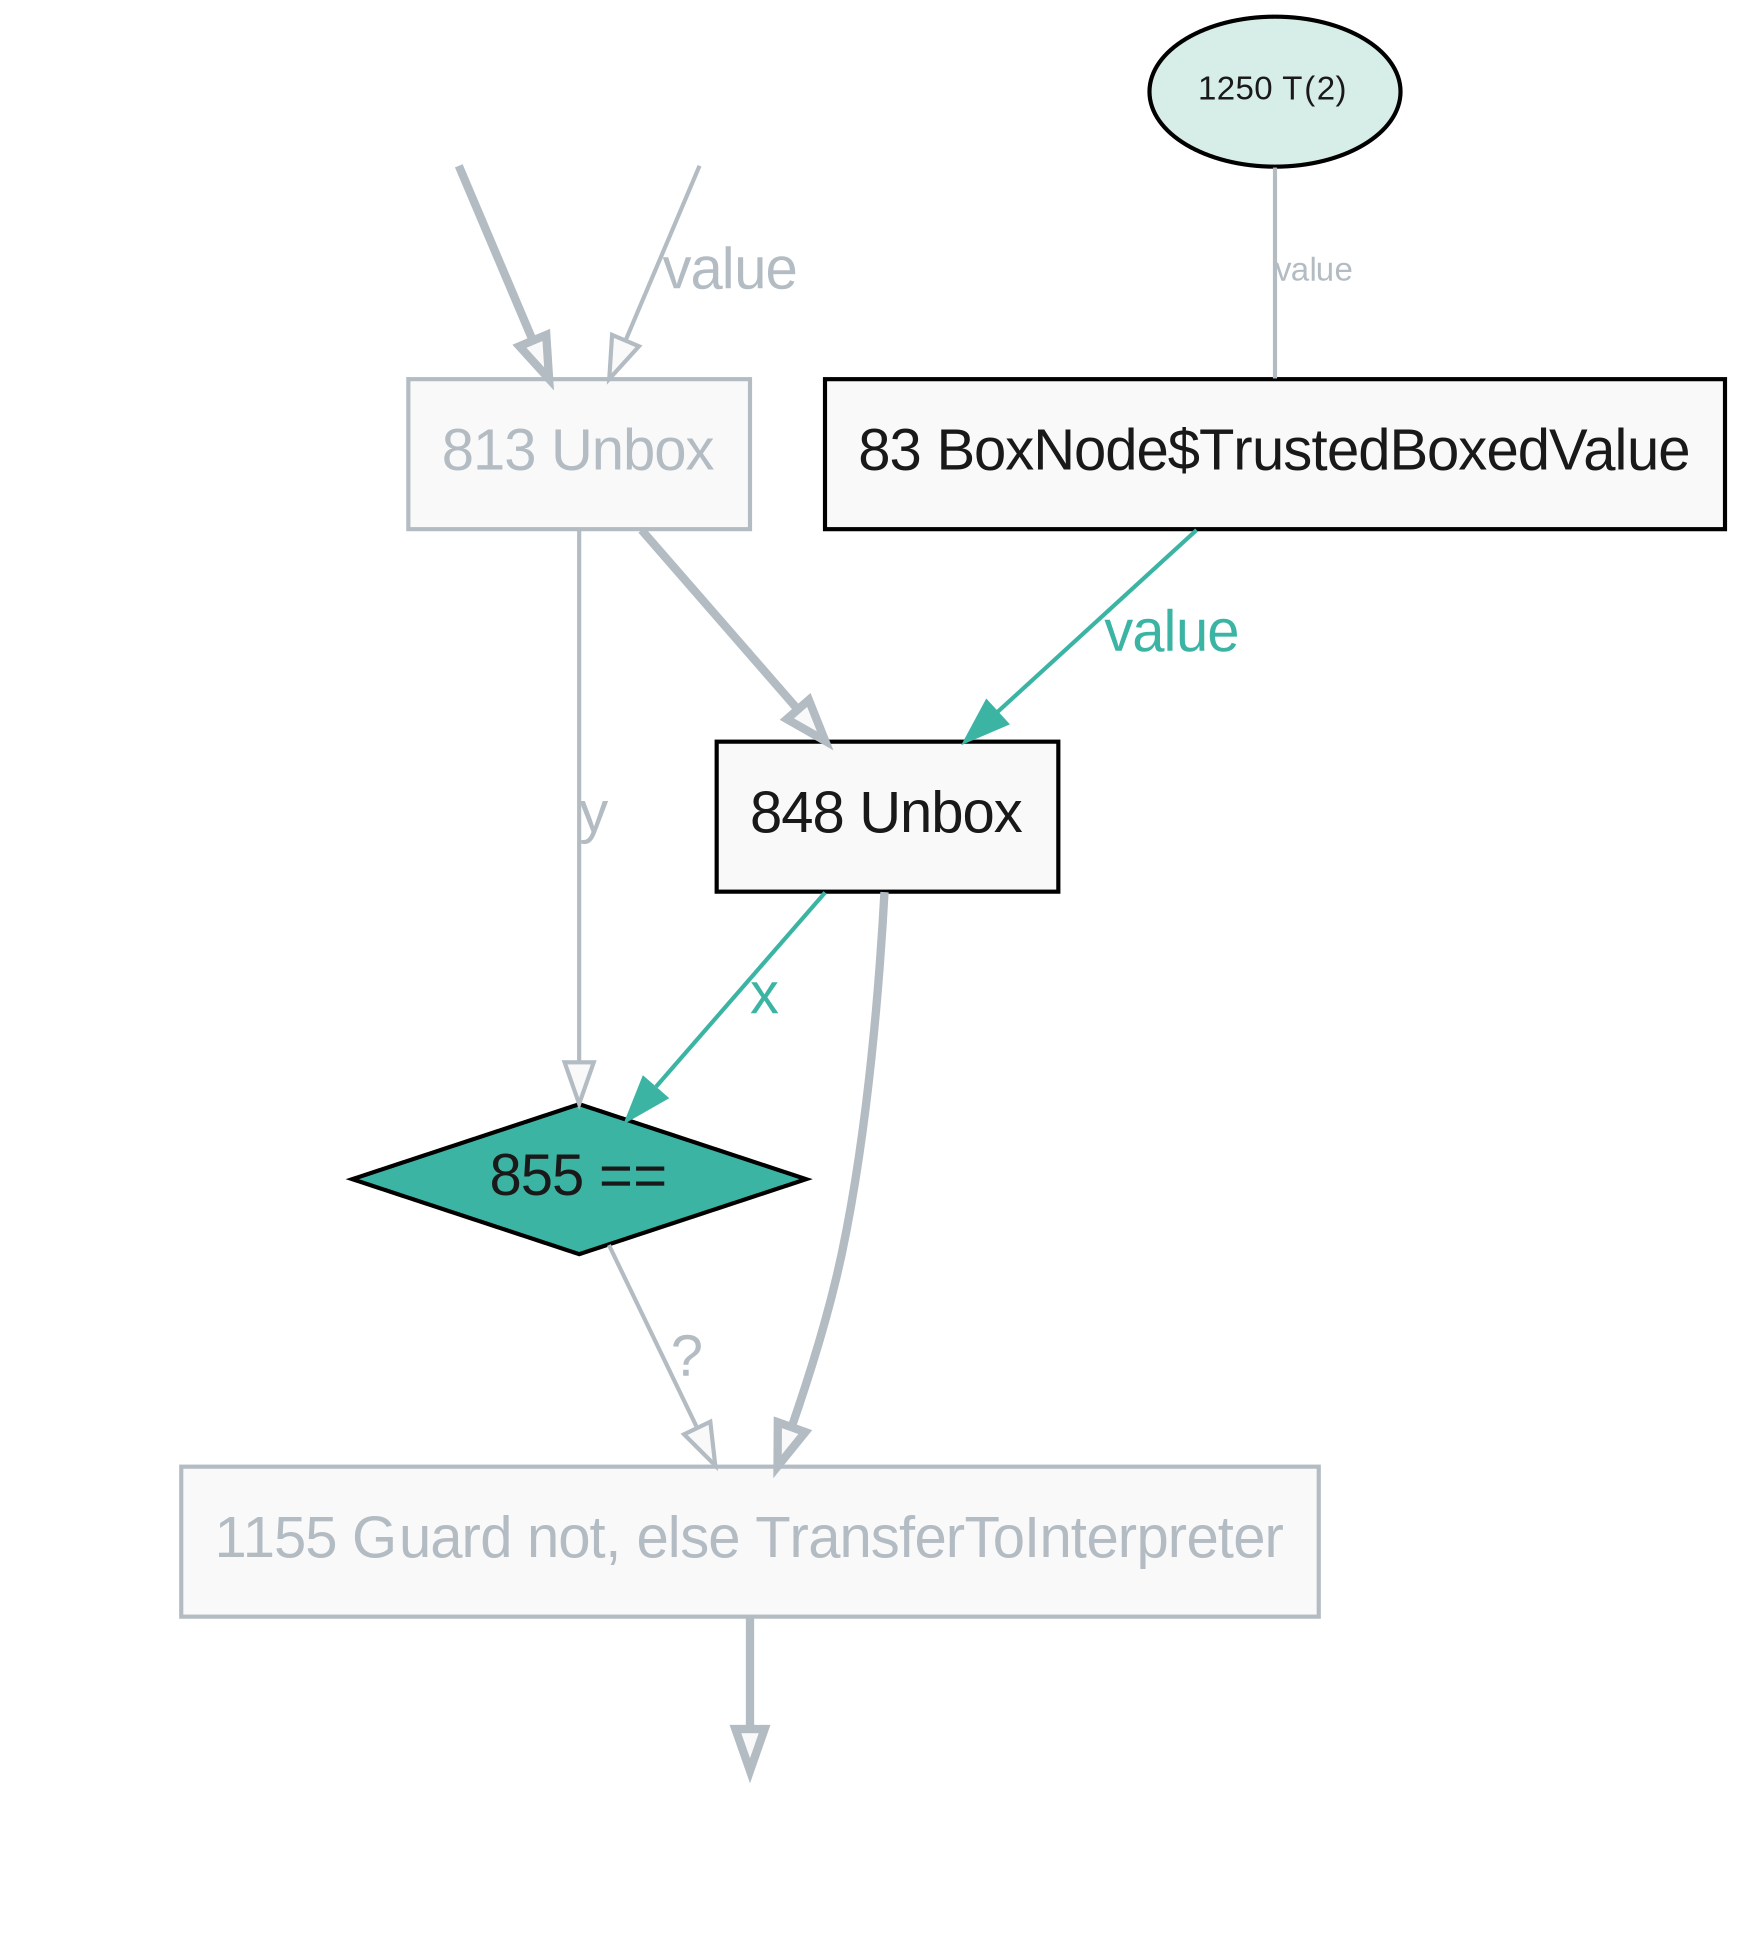
\includegraphics[width=0.4\textwidth]{figures/dot/List.contains.boxed-param-read.TruffleTier.png}
	\caption{Graal IR with speculative unboxing of \scalainline{elem} based on a type profile of its frame slot in \scalainline{List.contains}}
	\label{graalir:cons-contains-param-read}
\end{figure}

Truffle conveniently profiles the types of frame arguments to speculatively eliminate the unboxing of boxed values when reading frame values (including arguments).
Figure \ref{graalir:cons-contains-param-read} is an example of such a speculative optimization.
This speculative optimization relies on a \javainline{TrustedBoxedValue} to unbox the primitive.
A \javainline{TrustedBoxedValue} represents injected information from an external source.
In this particular case, it is known by the compiler that boxed instance comes from a cache; Unique \javainline{int} values may be mapped to a unique \javainline{Integer} instance in the Java runtime, which eliminates unnecessary boxed object creation.
The unbox operation in node $848$ will be `floated' up the graph such that all subsequent dominated by the read of a boxed frame value has no autoboxing.

In contrast, write operations of polymorphic frame values cannot be speculatively eliminated. 
Because Truffle does not specialize data layouts, i.e. frames are determined by their descriptors, which in turn are determined by the guest language implementation, frame writes of polymorphic values will always have to be boxed.
This is the main advantage when specializing the frame descriptor of a root node.
Code that has polymorphic code which reads and writes to a frame frequently will no longer have to unbox, compute primitive operations on unboxed values, then box those values back into their respective slots.
As our running example does not make use of this particular pattern of autoboxing, we will take this opportunity to showcase an instance of a polymorphic value read operation that Truffle is unable to speculatively optimize without specialization.

In both Scala and the JVM, arrays of primitive types are invariant with respect to the $\top$ (the universal supertype) type, \scalainline{Any} and \javainline{Object} in Scala and Java respectively.
That is to say, the type \scalainline{Array[Int]} is neither a subtype or supertype of the type \scalainline{Array[Any]}.
On the other hand, the type \scalainline{AnyRef} is covariant to the \scalainline{Array[Any]} type.
This contradiction in the presence of code which creates or operates on polymorphic arrays requires runtime bridge methods in order to appear seamless to the programmer.
These bridge methods combined with the nature of Scala's type system obscure opportunities for speculative optimizations.

\subsubsection*{Case Study: A List Constructor}

\begin{figure}[!htb]
	\begin{minted}{scala}
	object List {
		def apply[T](array: Array[T]): List[T] = {
			var i = array.length - 1
			var these: List[T] = Nil
			while (i >= 0) {
				these = new Cons[T](array(i), these)
				i -= 1
			}
			these
		}	
	}
	\end{minted}
	\caption{An alternate static constructor that converts an \scalainline{Array[T]} to a \scalainline{List[T]}}
	\label{impl:list-alt-constructor}
\end{figure}

To showcase an instance of when polymorphic array code must be bridged, we define an alternate constructor for a \scalainline{List[T]} to use an as example.
Figure \ref{impl:list-alt-constructor} gives a constructor that creates a polymorphic list from a polymorphic array.
We focus on the term \scalainline{array.length} which computes the length for a polymorphic array on line $3$.
When the Typer detects an array operation on a polymorphic array value, it automatically inserts the array runtime bridge method that is responsible for handling the operation.
For example, line $3$ after the Typer would be transformed into \scalainline{var i = array_length(array) - 1}.
We give the implementation of \scalainline{array_apply} in figure \ref{impl:array-length}.

\begin{figure}[!htb]
	\begin{minted}{scala}
	def array_length(array: AnyRef): Int = {
		if (array.isInstanceOf[Array[AnyRef]])       array.asInstanceOf[Array[AnyRef]].length
		else if (array.isInstanceOf[Array[Int]])     array.asInstanceOf[Array[Int]].length
		else if (array.isInstanceOf[Array[Double]])  array.asInstanceOf[Array[Double]].length
		else if (array.isInstanceOf[Array[Long]])    array.asInstanceOf[Array[Long]].length
		else if (array.isInstanceOf[Array[Float]])   array.asInstanceOf[Array[Float]].length
		else if (array.isInstanceOf[Array[Char]])    array.asInstanceOf[Array[Char]].length
		else if (array.isInstanceOf[Array[Byte]])    array.asInstanceOf[Array[Byte]].length
		else if (array.isInstanceOf[Array[Short]])   array.asInstanceOf[Array[Short]].length
		else if (array.isInstanceOf[Array[Boolean]]) array.asInstanceOf[Array[Boolean]].length
		else throw new NullPointerException
	}
	\end{minted}
	\caption{Implementation of \scalainline{array_length}}
	\label{impl:array-length}
\end{figure}

Notice the type of the argument in \scalainline{array_length} is \scalainline{AnyRef}; Because the types of primitive arrays and reference arrays are invariant, the direct supertype is \scalainline{AnyRef}.
To compute the length for a polymorphic, \scalainline{array_length} switch over every similar but unrelated array type.
In the body of every type check condition, the argument must be be cast to the appropriate array type after the type check succeeds before the length is finally computed.
We will examine how this code looks in the context of our alternate constructor after JIT compilation in Graal IR.

\begin{figure}
	\centering
	\includegraphics[width=\textwidth]{figures/dot/List.apply.boxed.array_length.png}
	\caption{Graal IR of \scalainline{array_length} in the context of \scalainline{List.apply[T](array: Array[T])}}
	\label{graalir:list-apply-boxed-array-length}
\end{figure}

Figure \ref{graalir:list-apply-boxed-array-length} contains the Graal IR of \scalainline{array_length} inlined into \scalainline{List.apply[T]}. 
Notice that the \scalainline{instanceof} type checks nodes (white) that are succeeded by an \javainline{ArrayLength} node (red) for each of the branches in \scalainline{array_length}.
The numerous consecutive conditional expressions complicate the control flow analysis in JIT compilation.
These conditional add unnecessary branching and burdens JIT compilation when the type of a specialized array should be known.
We introduce a method to vastly simplify the Graal IR of such instances of array bridge methods when specialized methods would have type-specific information to augment JIT compilation.

\begin{figure}[!htb]
	\begin{minted}{scala}
	import CompilerDirectives.castExact
	def copyArgumentsToFrame(frame: VirtualFrame): Unit = 
		for ((param, arg) <- params zip frame.getArguments) 
			param.tpe match {
				case Int =>
					frame.setInt(param.slot, arg.asInstanceOf[Int])
				...
				case Double =>
					frame.setDouble(param.slot, arg.asInstanceOf[Double])	
				case tpe: Array[AnyRef] | tpe: Array[Int] | ... | tpe: Array[Double] =>
					frame.setObject(param.slot, castExact(arg, getClass(tpe)))
				case _ =>
					frame.setObject(param.slot, arg)
			}
	\end{minted}
	\caption{Pseudocode for \scalainline{DefDefNode} and \scalainline{Parameter}}
	\label{impl:specialized-copy-arguments}
\end{figure}

In order to accomplish this, we extend the way that frame arguments are copied into the frame from figure \ref{impl:defdefnode}.
Because a parameter now retains its type instead of a frame slot kind, we introduce a special operation when copying arguments that are arrays. 
The \javainline{castExact} directive is a type narrowing operation that hints to Graal that a value is an instance of a type.
We will examine how the insertion of this directive for array types simplify the layout of Graal IR graphs.

\begin{figure}[!htb]
	\centering
	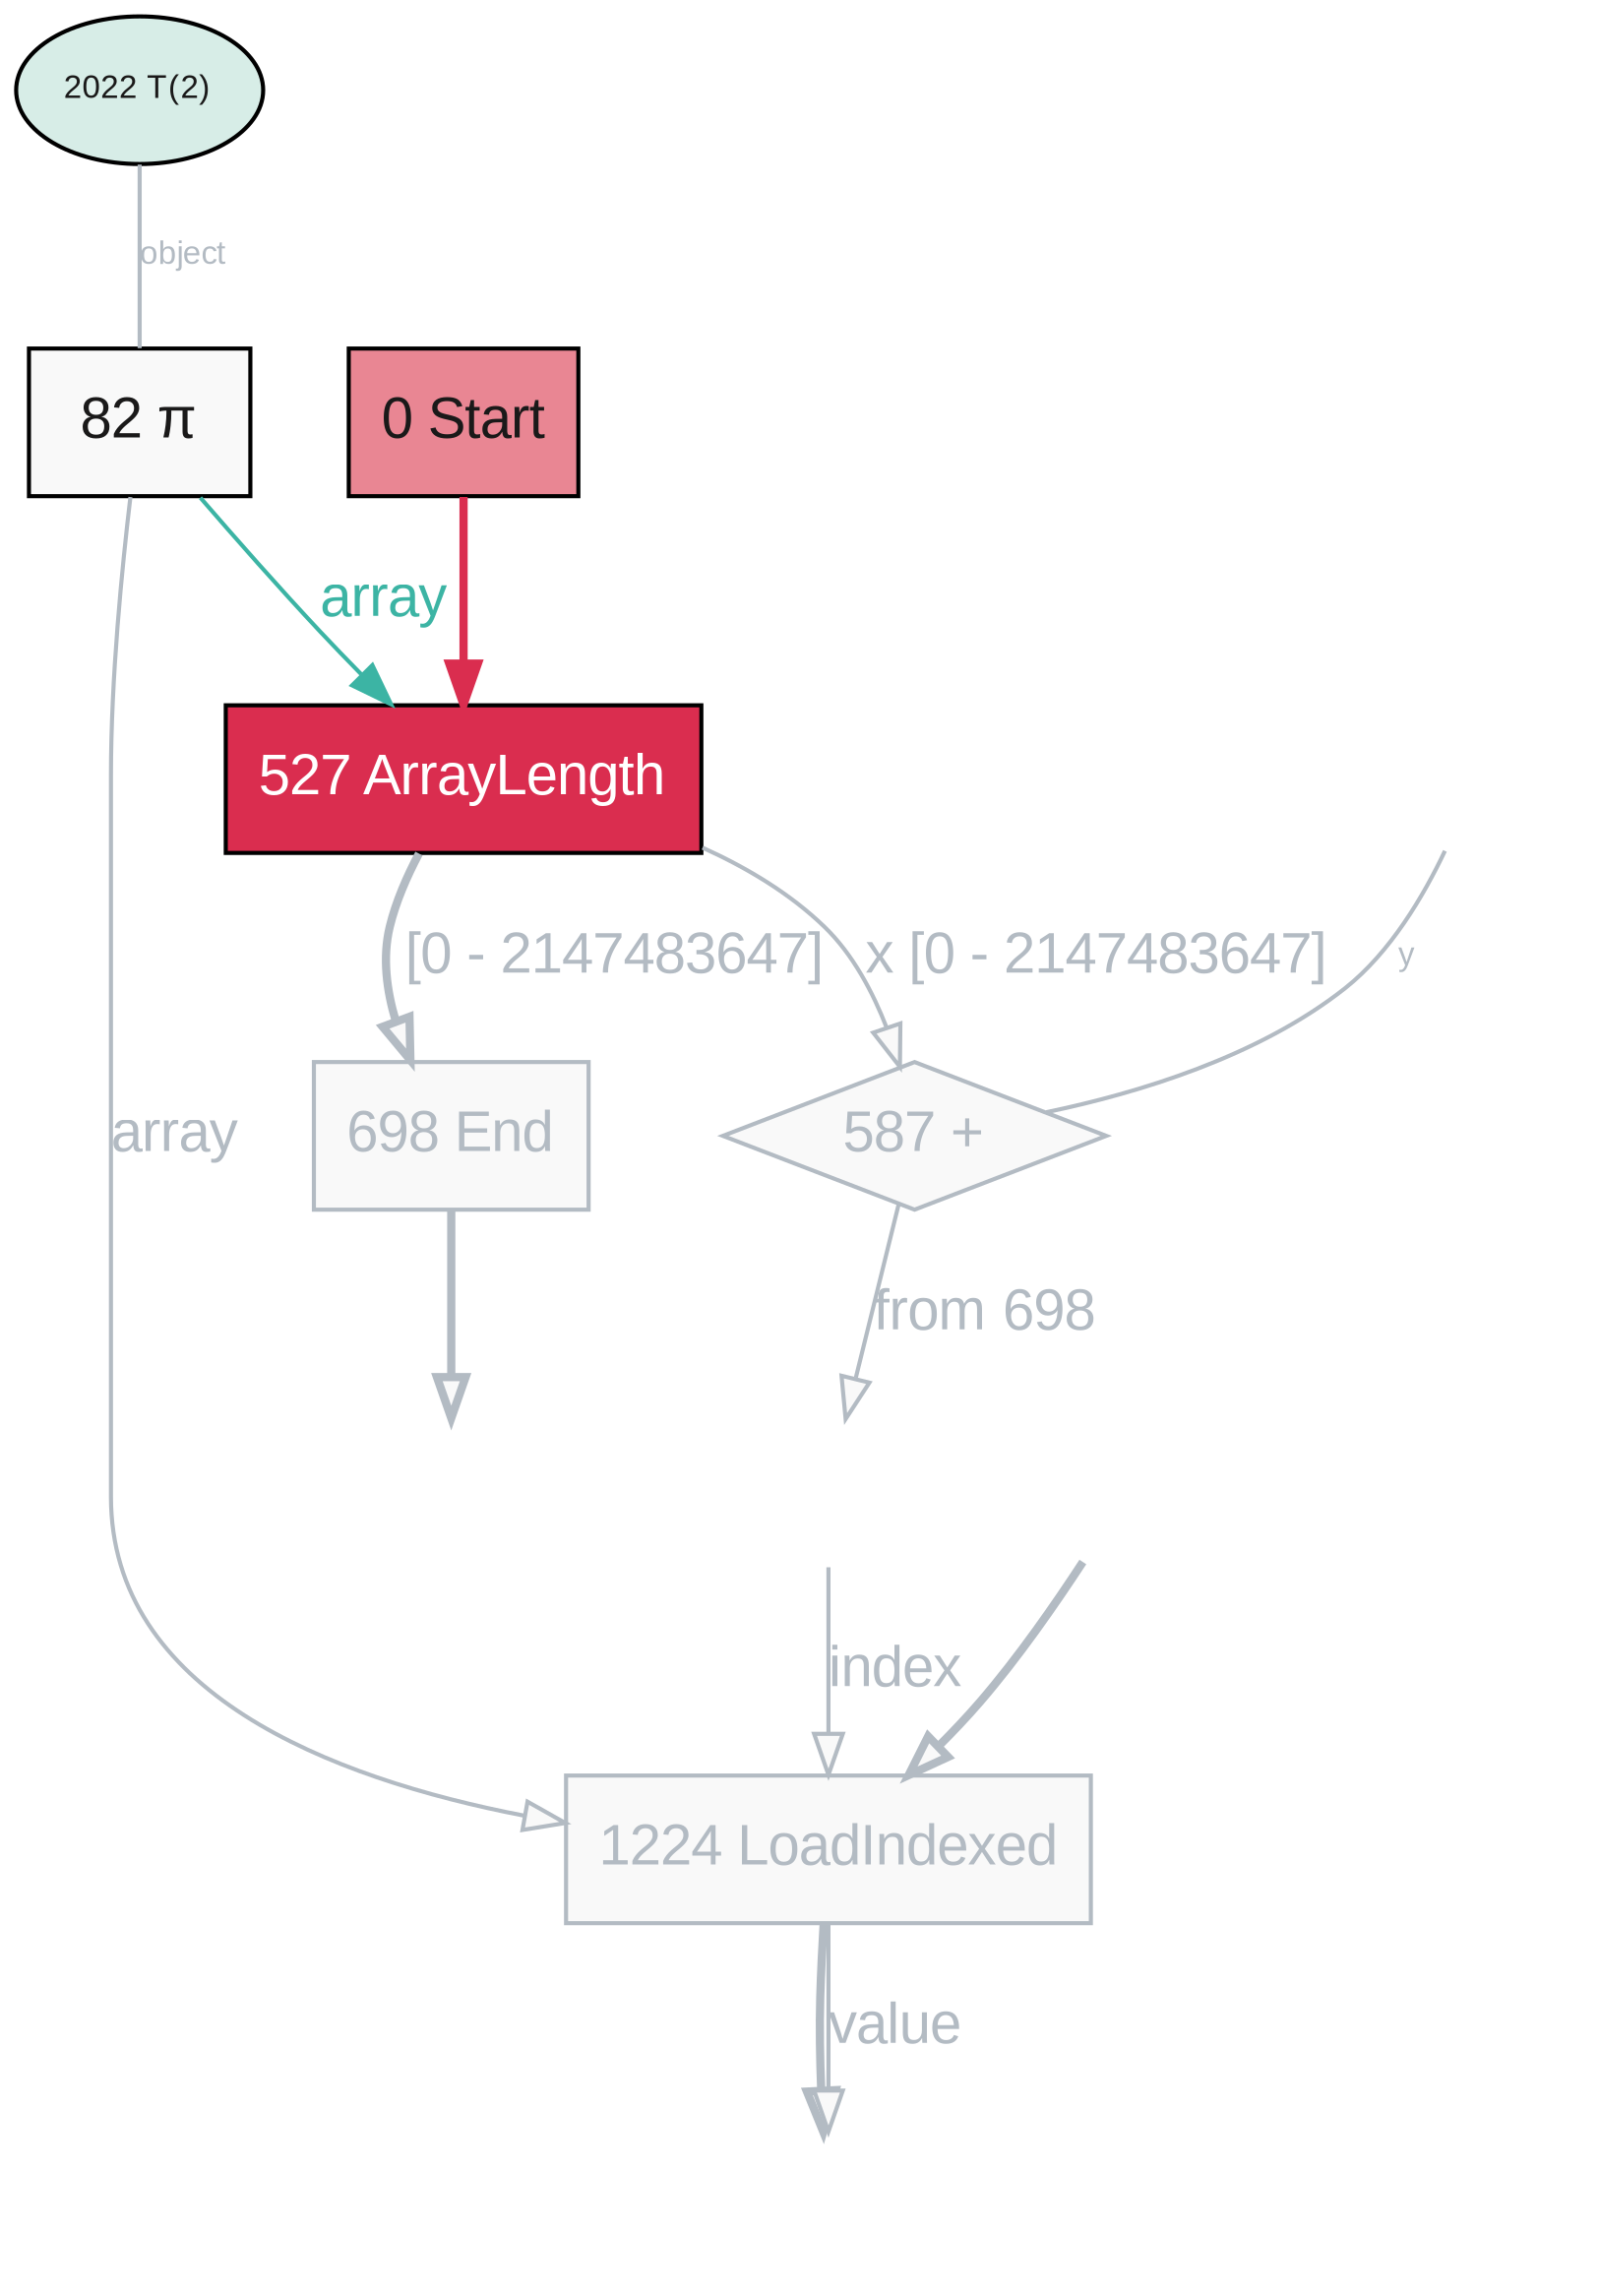
\includegraphics[width=0.3\textwidth]{figures/dot/List.apply.specialized.array_length.png}
	\caption{Graal IR of \scalainline{array_length} in the context of \scalainline{List.apply[T](array: Array[T])} augmented with a $\pi$ node}
	\label{graalir:list-apply-specialized-array-length}
\end{figure}

Figure \ref{graalir:list-apply-specialized-array-length} contains the simplified Graal IR of \scalainline{array_length} inlined into \scalainline{List.apply[T]}.
Notice that there is a single \javainline{ArrayLength} node that is dominated by a $\pi$ node.
A $\pi$ node\cite{abdc:pi-nodes} enforce a bound on value.
In the case of Graal, a $\pi$ node enforces bound on the type of a value.
More specifically in our example, the $\pi$ node narrows the type of the 2nd parameter of \scalainline{List.apply[T]} to a monomorphic array type.
When the type of the parameter is narrowed, the type checks that enforce array types from figure \ref{graalir:list-apply-boxed-array-length} are eliminated because the type is now known.

This method does not consider polymorphic scenarios where an array of boxed primitives are used interchangeably with an array of primitives.
Such scenarios would require the insertion of additional autoboxing nodes or an intraprocedural transformation where boxed arrays are converted to primitive arrays.
While these solutions are possible in the context of Truffle, we consider these kinds of scenarios out of the scope of this thesis.

\subsubsection*{Invoking Polymorphic Methods}

\begin{figure}[!htb]
	\begin{minted}{scala}
	def parseApply(apply: Apply): ApplyNode = {
		val signature = apply.symbol.signature
		apply match {
			case Apply(Select(qualfier, _), arguments) => ... // monomorphic trees
			case Apply(TypeApply(Select(qualifier, _), targs), args) =>
				new ApplyNode(signature, parse(qualifier), (targs ++ args).map(parse))
		}
	}
	\end{minted}
	\caption{Extension to parsing a polymorphic \scalainline{Apply} tree.}
	\label{impl:parse-typeapply}
\end{figure}

So far we have shown how to create a specialized method, but not when to create one.
For this demonstration, we will show one of the natural benefits of executing TASTy (and other high level intermediate representations).
A polymorphic method invocation in TASTy is always an \scalainline{Apply} tree node where the qualifier is a \scalainline{TypeApply}.
The \scalainline{TypeApply} tree node represents a \textit{type application}.
Without delving into great detail, a type application is the process of producing a monomorphic method from a polymorphic method by matching type parameters to type arguments.
Analogous to normal applications which accept values as arguments and produces values as results, type applications accept types as arguments and produce types as a result.
With this in mind, \scalainline{TypeApply} nodes are a naturally suitable site to invoke and create specializations for methods.

Figure \ref{impl:parse-typeapply} extends the transformation of \scalainline{Apply} tree nodes to include polymorphic applications.
The application of a polymorphic method follows the same semantics as the application of a monomorphic method.
The actual specialization of the frame layout occurs inside the template that a polymorphic \scalainline{ApplyNode} invokes.
This allows the invocation of polymorphic methods even in the presence of dynamic dispatch.
In the next section, we will describe additional machinery that is added \textit{after} a polymorphic inline cache has resolved virtual dispatch to handle type application and how to make such mechanisms amenable to partial evaluation.

\subsubsection*{Typed Dispatch Chains}

\begin{figure}[!htb]
	\begin{minted}{scala}
	class DefDefTemplate(...) extends RootNode(...) { 
			
		@CompilerDirectives.CompilationFinal
		val specializations: Array[(Array[Type], DirectCallNode)] = Array.empty
			
		def execute(frame: VirtualFrame): Object = {
			val typeArguments = resolveArguments
			dispatchCached(frame, types)
		}
			
		@ExplodeLoop
		def dispatchCached(frame: VirtualFrame, typeArguments: Array[Type]): Object = {
			for ((typeSignature, specialization) <- specializations)
				if (typeSignature == typeArguments)
					return specialization.call(frame.getArguments)
			CompilerDirectives.transferToInterpreterAndInvalidate()
			dispatchNew(frame, typeArguments)
		}
		
		def dispatchNew(frame: VirtualFrame, typeArguments: Array[Type]): Object = {
			val specialization = specialize(typeArguments)
			val callNode = DirectCallNode.create(specialization)
			specializations += (typeArguments -> callNode)
			callNode.call(frame.getArguments)
		}
		
		...
	}
	\end{minted}
	\caption{Pseudocode for typed dispatch inside a \scalainline{DefDefTemplate}.}
	\label{impl:defdeftemplate-execute}
\end{figure}

Dispatch chains\cite{trufflyruby:specialization} are multi-layered inline caches.
We introduce the notion of \textit{typed dispatch chains}.
Typed dispatch chains integrate the semantics of type applications onto the execution mechanism of a root node.
Figure \ref{impl:defdeftemplate-execute} contains the simplified implementation of the execution semantics in a \scalainline{DefDefTemplate}.

Specializations of polymorphic methods are created on demand then cached based on their type signatures.
One particular challenge of making caching mechanism fold away in partial evaluation is that the cache must be a \textit{compilation constant}.
Truffle provides the \javainline{CompilationFinal} directive which indicates that a value which may not be a constant in the guest language implementation \textit{will} be a constant when being partially evaluated.
Type arguments at type application sites are always stable, i.e. their respective type nodes evaluate to the same type, the look up of the specialized call node should have no overhead when JIT compiled with aid of partial evaluation. 
To make this possible, we exploit a simple array of type signature and specialized call node pairs.
When the loop for looking up a cache entry in the array is unrolled during partial evaluation (directed by \javainline{ExplodeLoop}), the loop is transformed into a block of conditional expressions for each cache entry.
This unrolled loop combined with the injected knowledge that type argument values are compilation constants results in the conditional elimination\cite{conditional-elim} of entries other than the correct corresponding cache entry.

When a combination of type arguments have not yet been encountered and their corresponding specialization is unavailable, the specialization must be generated and then invoked.
To prevent this \textit{slow} path of execution from being JIT compiled, we direct the compiler using \textit{bail out} of JIT compilation with the \scalainline{transferToInterpreterAndInvalidate} directive.
The directive allows guest languages to insert their own deoptimization into the control flow of a program.
This ensures compiled code of the slow branch when creating the specialization is never compiled.
Note that in the first case where a type argument lookup succeeds (the fast path), the directive is unreachable because the control flow of the code returns and therefore will not be part of compiled code.

\begin{figure}[!htb]
	\centering
	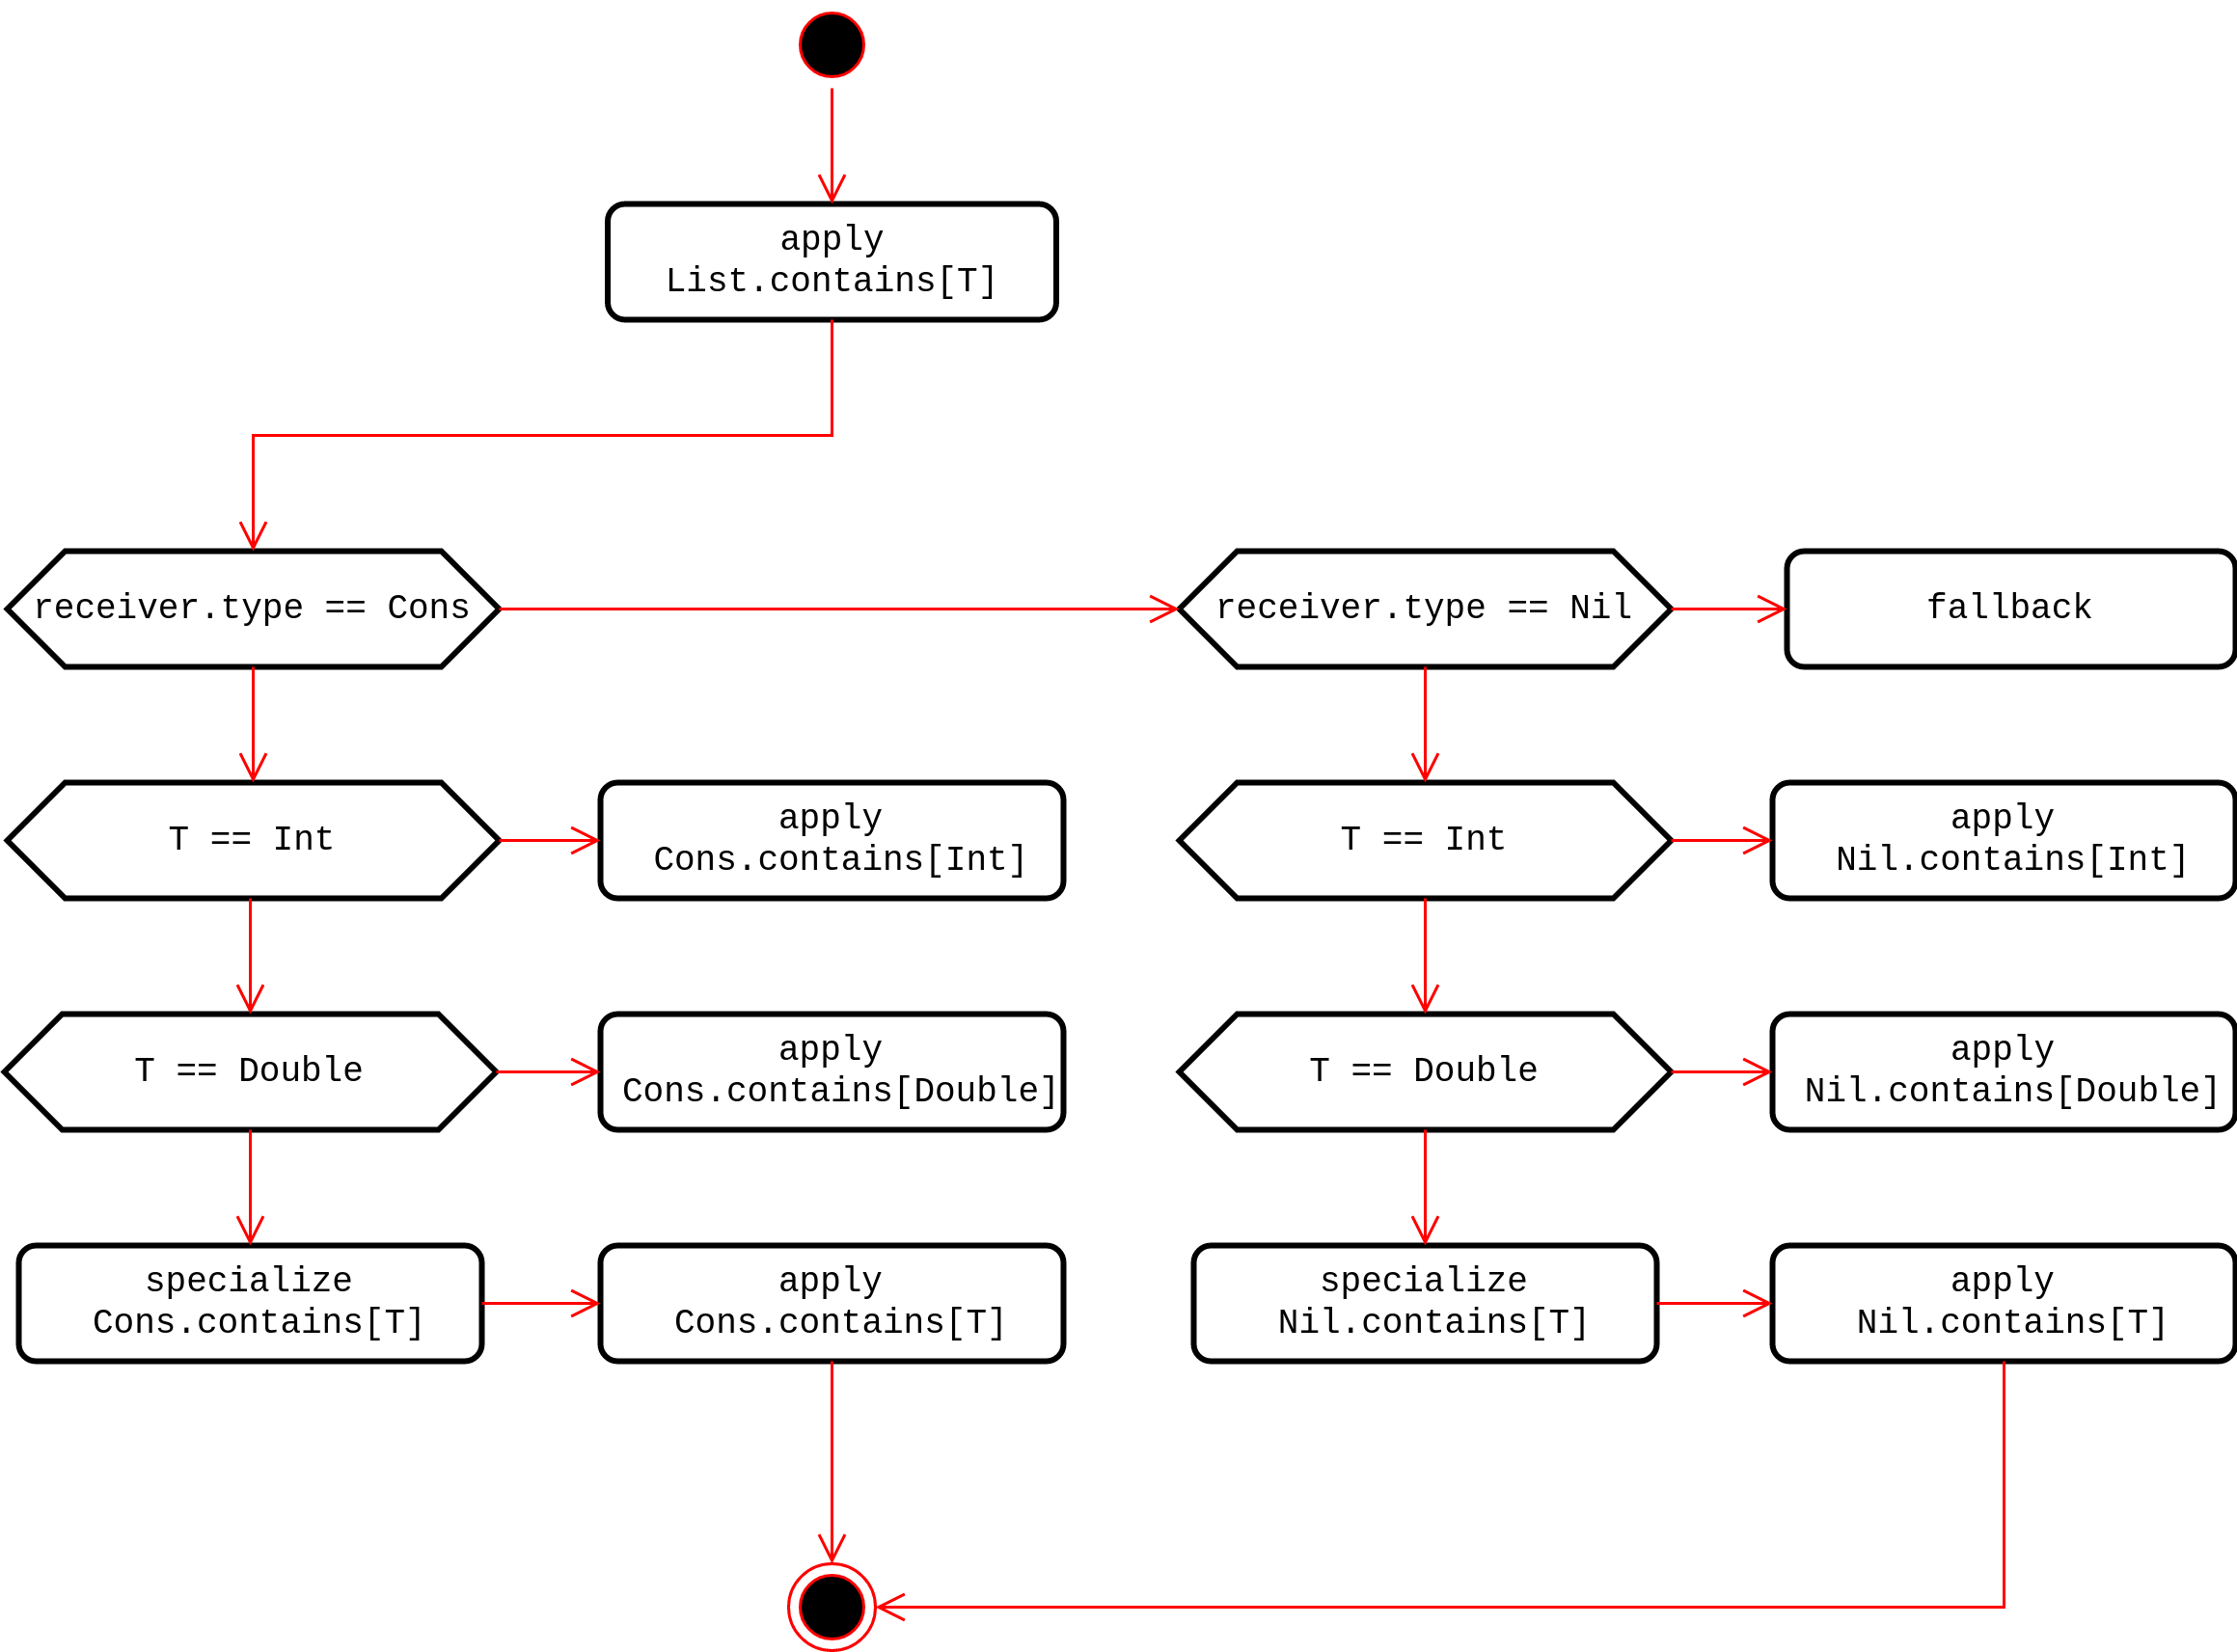
\includegraphics[width=0.75\textwidth]{figures/tastytruffle-type-dispatch-chain.png}
	\caption{The typed dispatch chain for a \scalainline{List.contains} call site}
	\label{example:typed-dispatch}
\end{figure}

Figure \ref{example:typed-dispatch} is an extension of the example given in figure \ref{example:poly-cache-call-node} with typed dispatch.
The example assumes the type arguments for \scalainline{Int} and \scalainline{Double} for \scalainline{Cons.contains[T]} and \scalainline{Nil.contains[T]} has previously been specialized and cached.
After the polymorphic inline cache resolves the receiver to an exact type, the corresponding specialization is looked up.

\subsection{Specializing Classes}

We begin with a discussion on specializing classes as they can only be polymorphic under a single context.
This is in contrast to methods, which can be polymorphic under multiple contexts.
In this section, we specifically focus on specializing classes and their members which solely derive their polymorphic semantics from class type parameters.

\begin{figure}[!htb]
	\begin{minted}{scala}
	class NewNode(@Child typeNode: TypeNode) extends TermNode {
		override def execute(frame: VirtualFrame): Object = {
			val tpe = typeNode.resolveType(frame)
			shapeOf(tpe).newInstance
		}
	}
	\end{minted}
	\caption{The \scalainline{NewNode} for the polymorphic interpreter.}
\end{figure}

\subsubsection*{Case Study: \texttt{Cons.head}}

\begin{figure}[!htb]
	\begin{minted}{scala}
	val list: List[Int] = ???
	list.contains(0)
	\end{minted}
	\caption{Example invocation of \scalainline{Cons.contains[Int]}}
\end{figure}

We introduce an example which will motivate the specialization of storage layouts in shapes.

\begin{figure}[!htb]
	\centering
	\begin{subfigure}[b]{0.4\textwidth}
		\centering
		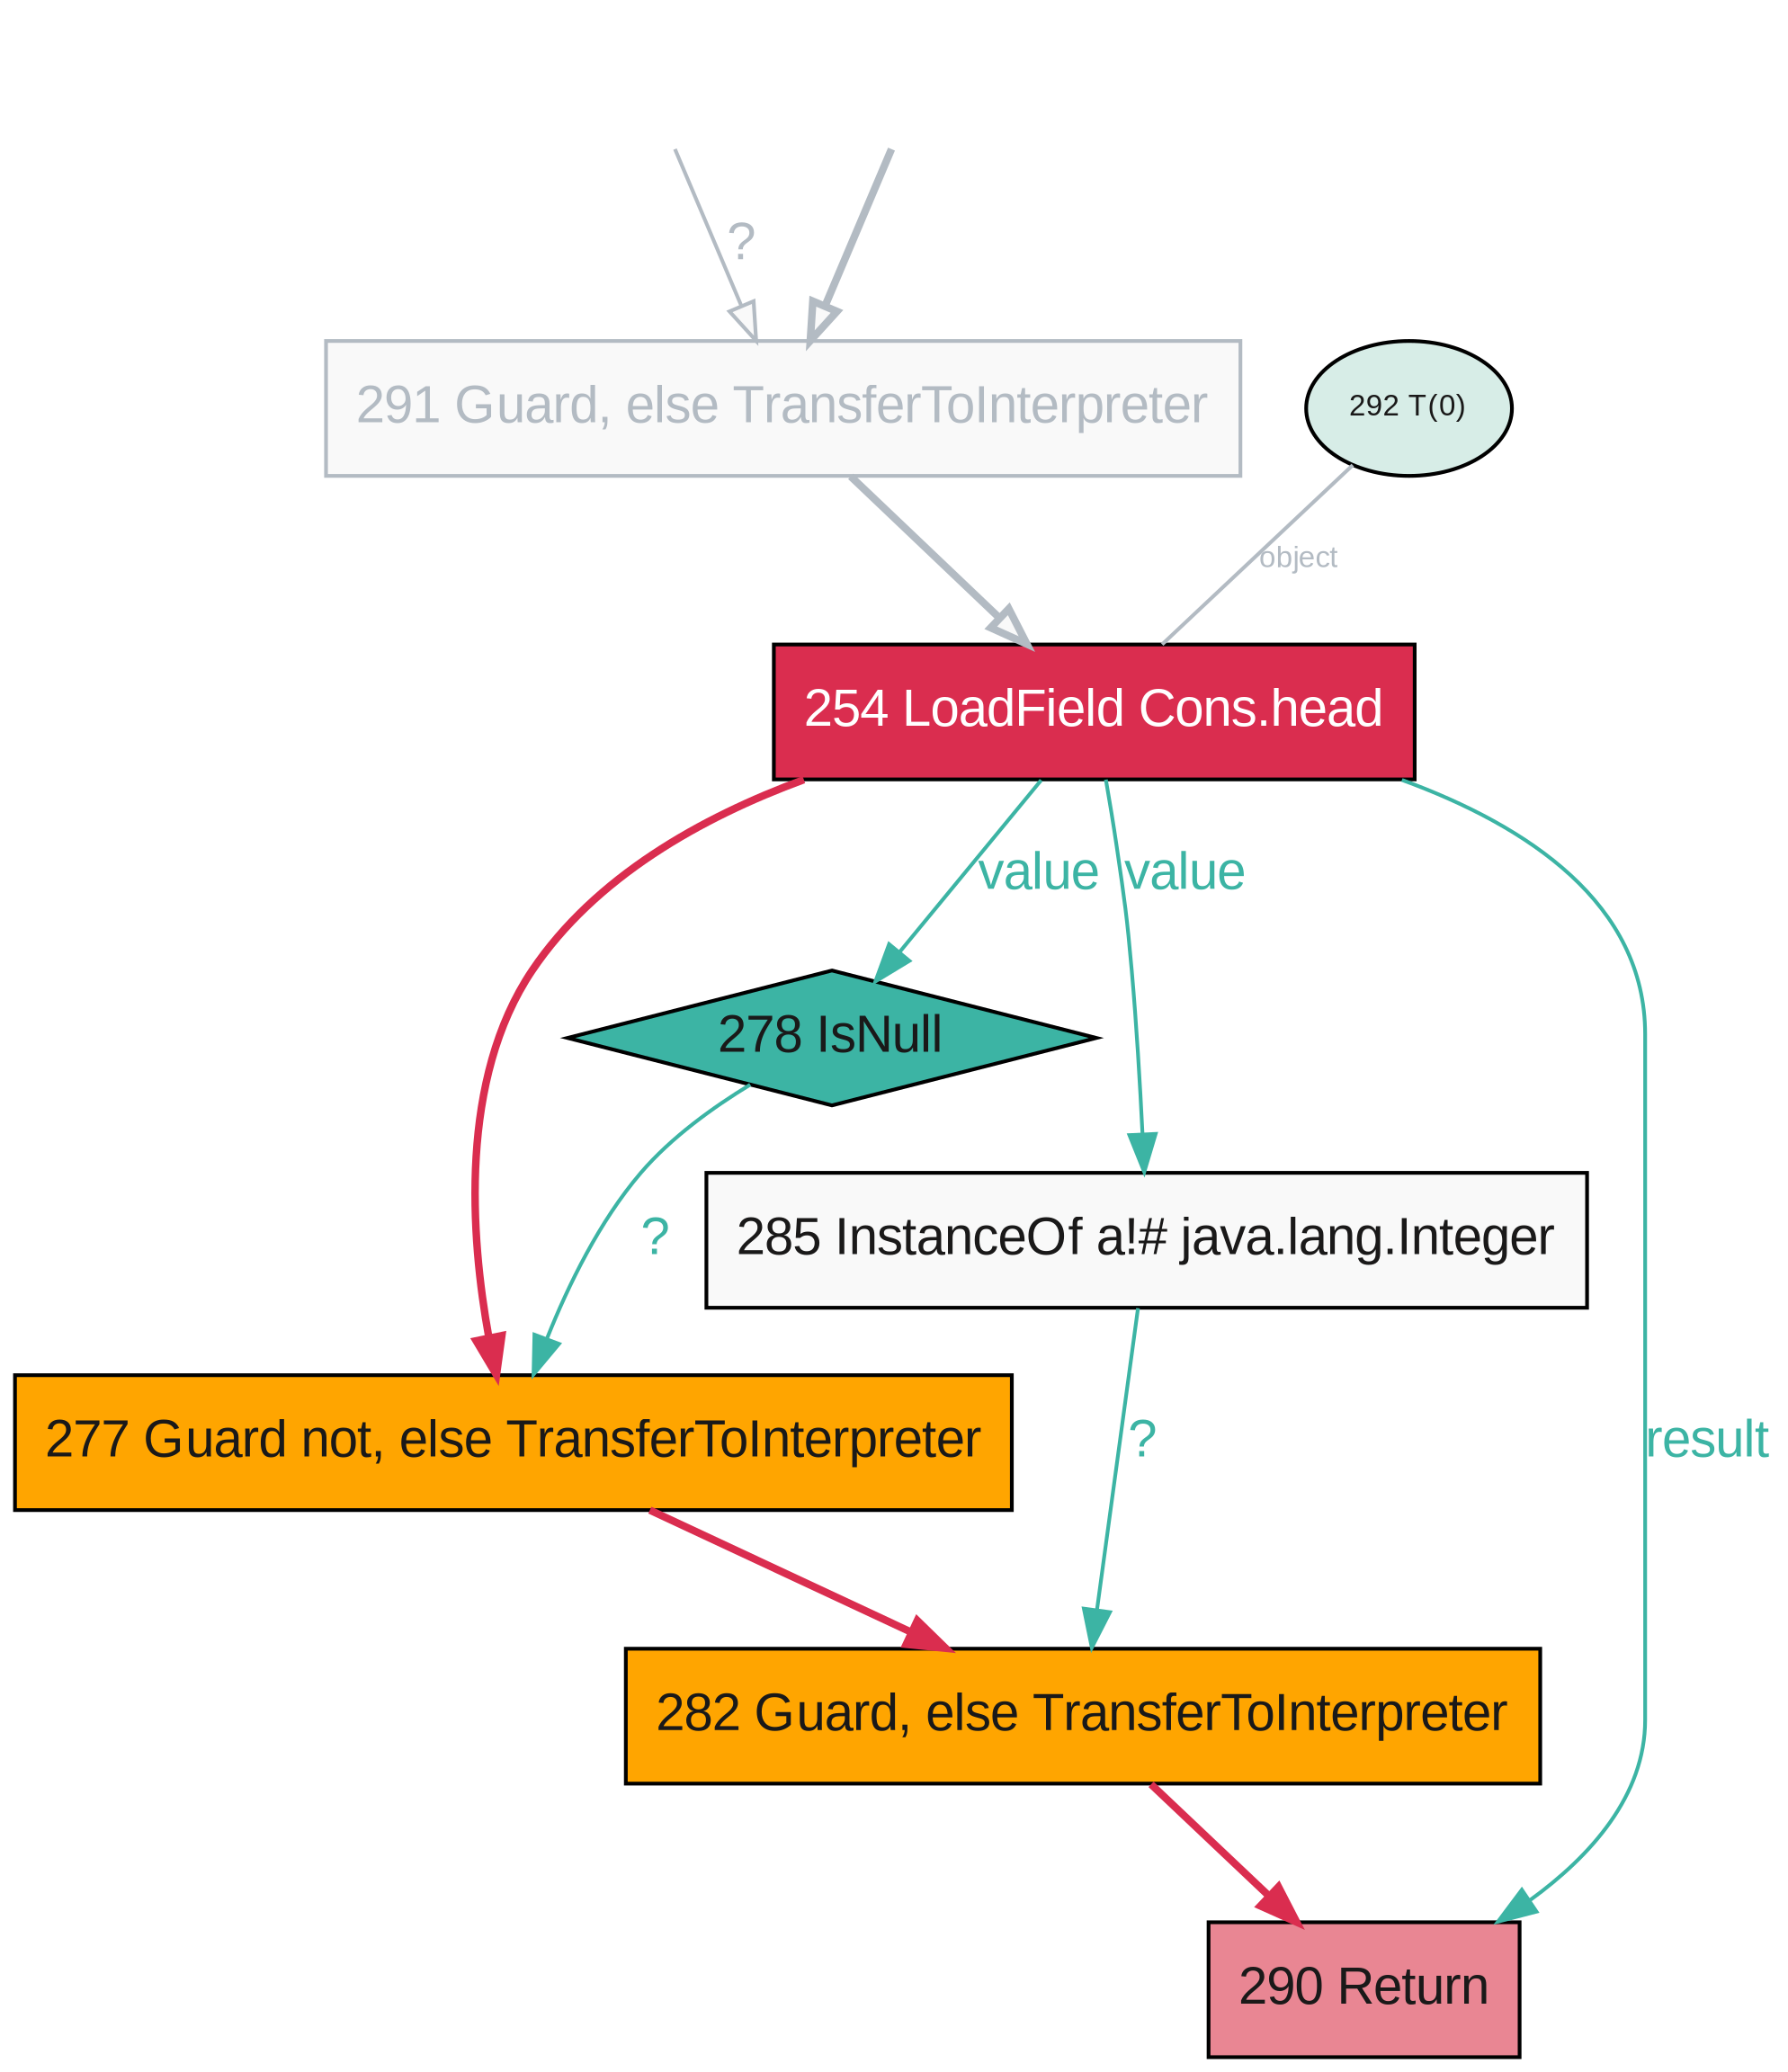
\includegraphics[width=\textwidth]{figures/dot/List.head.boxed.TruffleTier.png}
		\caption{Graal IR of \scalainline{Cons.head} focused on field access of \scalainline{head0}}
		\label{graalir:cons-head-boxed}
	\end{subfigure}
	\hfill
	\begin{subfigure}[b]{0.45\textwidth}
		\centering
		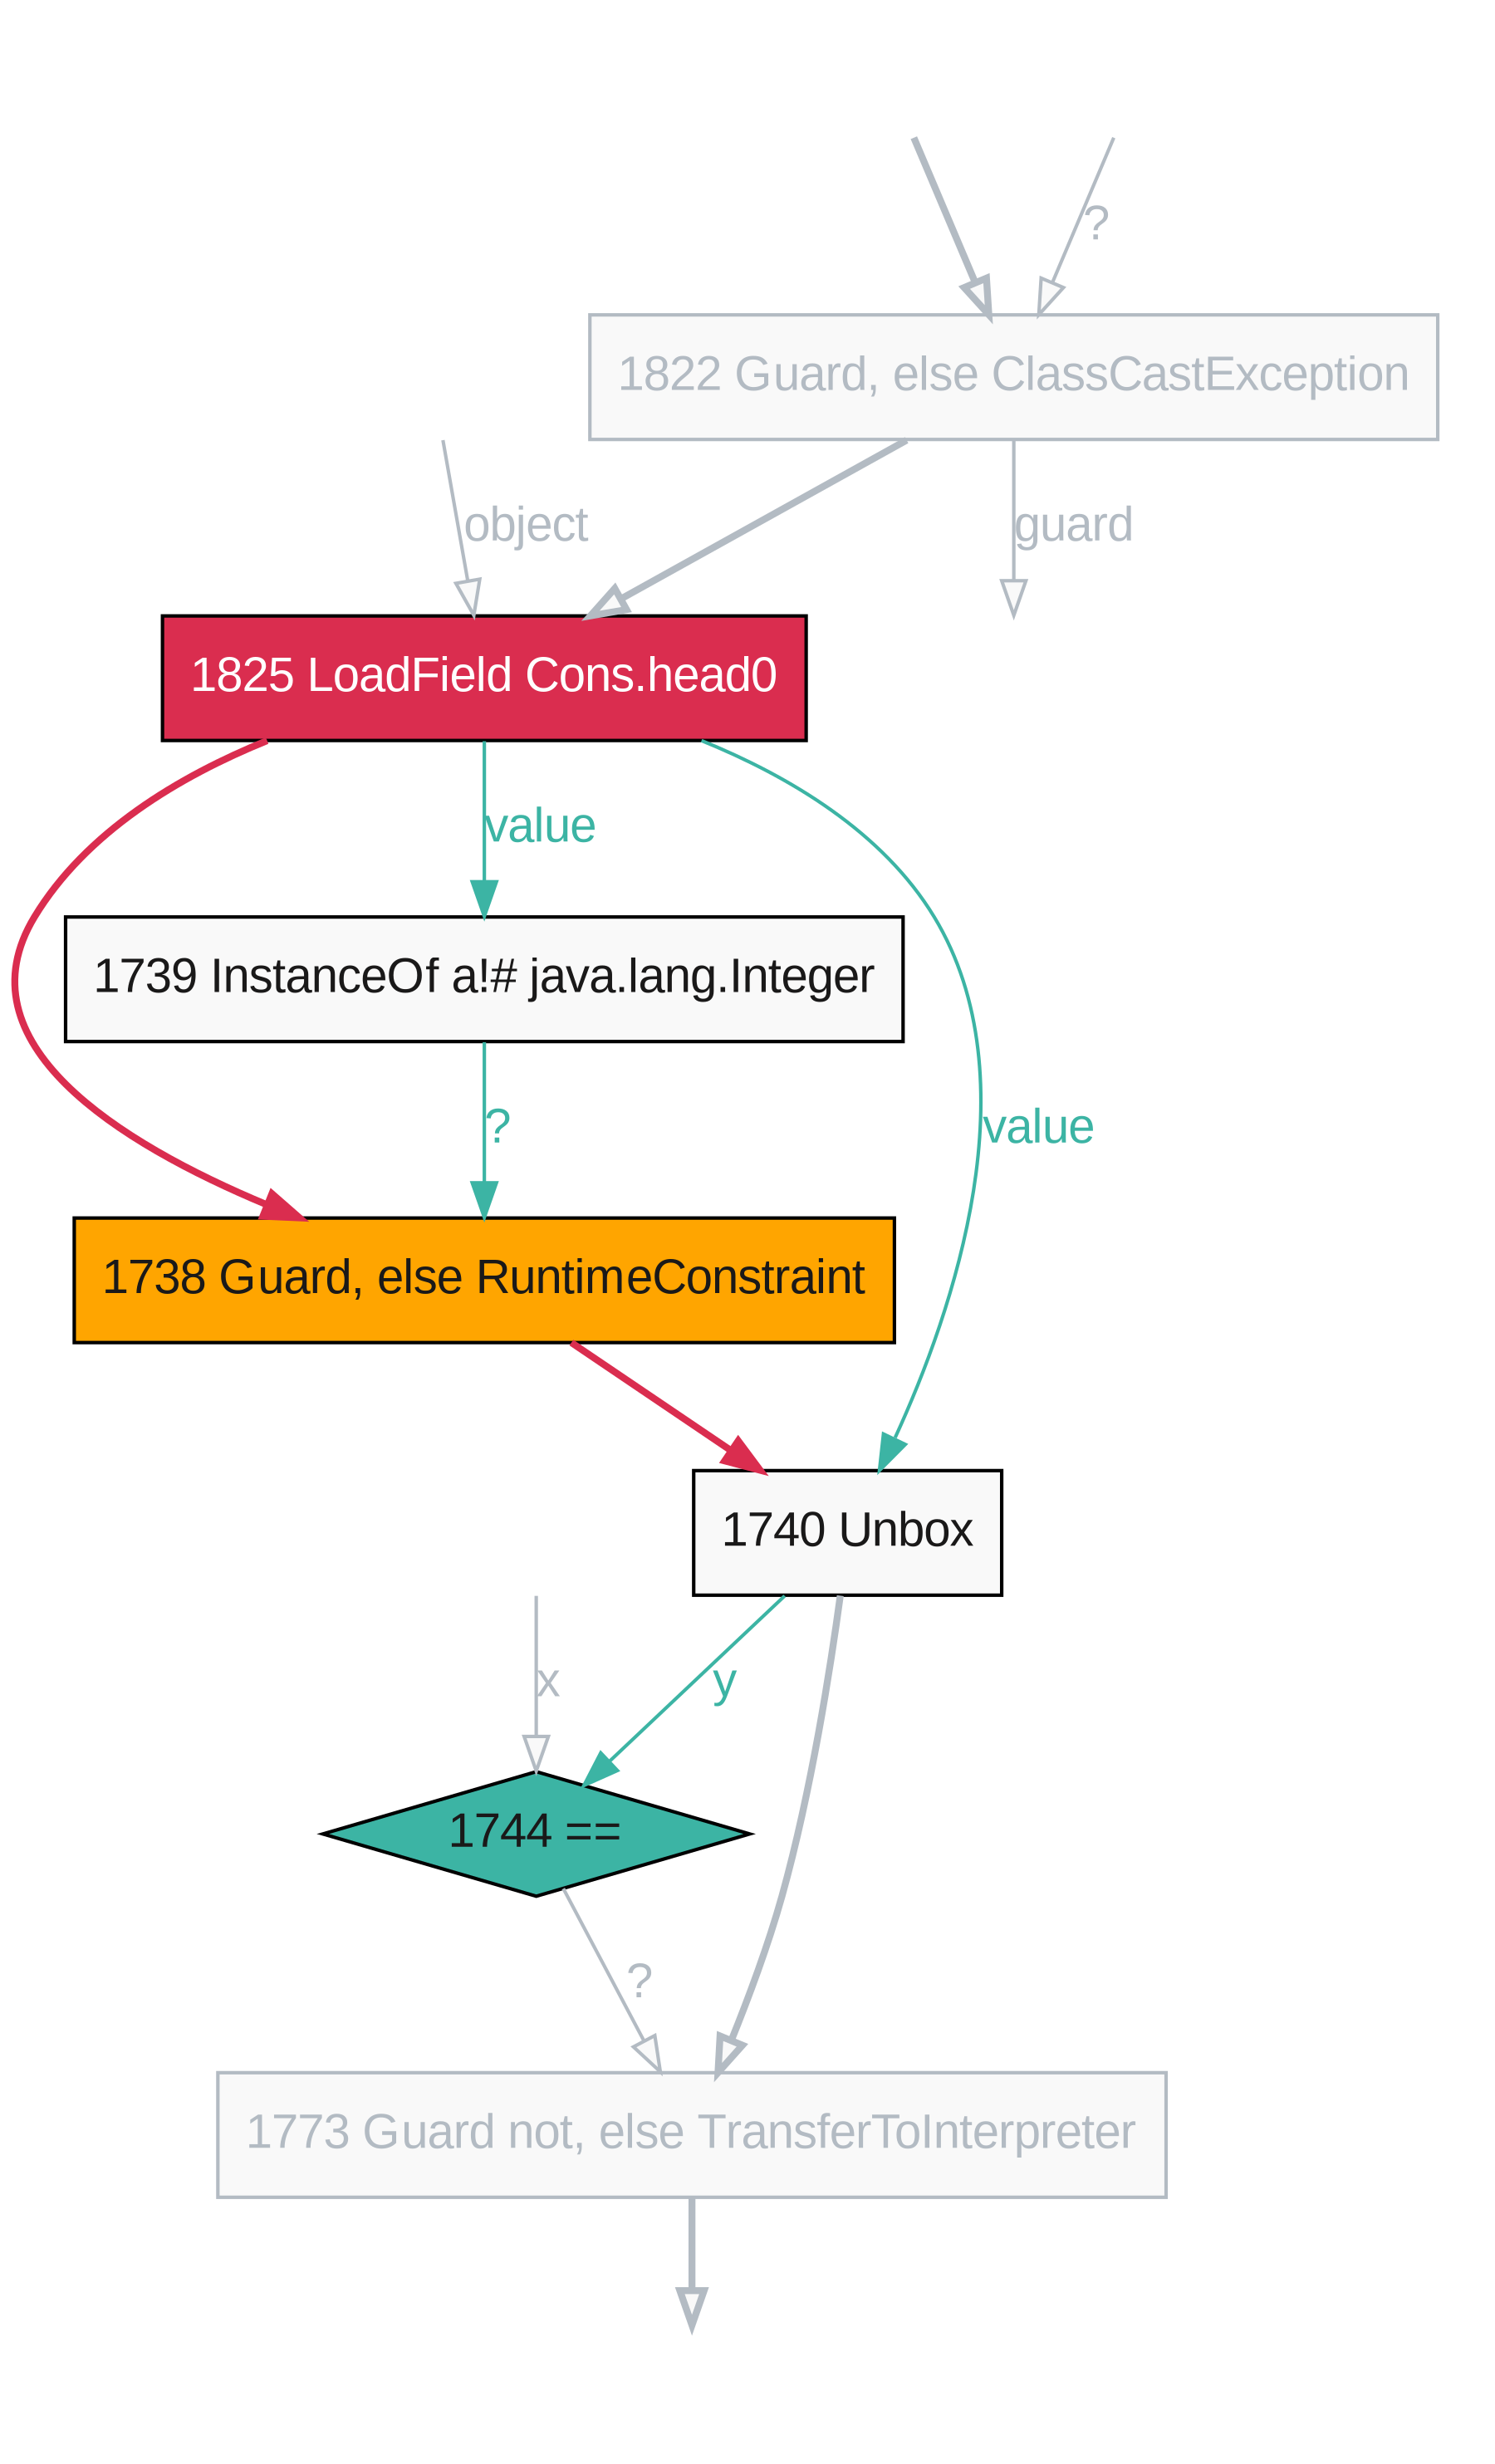
\includegraphics[width=\textwidth]{figures/dot/List.contains.boxed.TruffleTier.png}
		\caption{Graal IR of \scalainline{Cons.head} after being inlined into \scalainline{Cons.contains}}
		\label{graalir:cons-contains-head-focus-boxed}
	\end{subfigure}
	\hfill
\end{figure}

We examine in detail the Graal IR focusing on the \scalainline{List.head} accessor method in our \scalainline{List} running example.
For this particular example, we focus on unboxing that occurs when the \scalainline{head0} is accessed by the \scalainline{List.head}.
This unboxing can be seen in \ref{graalir:cons-head-boxed}.

We can see that \textit{guard} nodes are inserted by Graal into the compiled graph during JIT compilation.
A guard node ensures a speculative assumption still holds during execution.
Because the default storage type of a polymorphic field without specialization is an \javainline{Object}, Graal makes two runtime assumptions about the field in the JIT compiled \scalainline{contains} method to ensure the compiled method does not throw a runtime exception if the return value needs to be unboxed.
The first guard, identifiable by node $278$, checks that the value is not the \javainline{null} reference.
As the \javainline{null} value is only compatible with reference types, attempting to unbox a \javainline{null} value produces a runtime exception.
The second guard, with the identifier $282$, is a type check that the value is an \javainline{Integer} object.
Notice that the predecessor node is the type check \javainline{instanceof a!{\#} java.lang.Integer} and not \javainline{instanceof java.lang.Integer}.
\javainline{instanceof} nodes in Graal IR checks against \textit{stamps} instead of normal JVM types identifiers.
A stamp is much like a type identifier but has additional descriptors attached.
For example, the stamp \javainline{a!{\#} java.lang.Integer} has the following descriptors:

\begin{description}
	\item[\texttt{(a)}] Asserts that the stamp marks a reference type identifier. In the case of this stamp, the stamp marks the boxed reference type \javainline{java.lang.Integer}.
	\item[\texttt{(!)}] Asserts that value is not the \javainline{null} reference value. The stamp contains this descriptor because it is preceded by a non-null guard.
	\item[\texttt{(\#)}] Asserts that value marked by the stamp is \textit{exactly} an instance of the type identifier described by the stamp and not an instance of a subclass of the type identifier
\end{description}

In more succinct terms, the \javainline{instanceof} node $285$ checks that value is precisely the instance of a \javainline{java.lang.Integer} and is not the \javainline{null} value. 
If the assumptions are not violated in compiled code, the boxed integer value is then returned from the compiled code.
Note that no unboxing happens because the value of \scalainline{head0} has not yet been used in a polymorphic context.

When the access or method \scalainline{List.head} is inlined into its callsite in \scalainline{Cons.contains} (see figure \ref{graalir:cons-contains-head-focus-boxed}), an unbox operation is introduced because the equality operation in node $1744$ compares primitives and not references.
Notice that the two guards node previously seen in figure \ref{graalir:cons-head-boxed} are folded into one node because the \javainline{instanceof} node is an extension of the null check node.
Because polymorphic field values are stored as an reference on the object instance, these speculative assumptions are necessary in order to generate compiled code.
To eliminate the overhead of the unbox operation and the accompanying guard nodes, The polymorphic fields of a class must be specialized.

\subsubsection*{Specializing Field Members}

The underlying type of a polymorphic field, and therefore its storage type as part of the shape layout, cannot be determined statically.

\begin{figure}[!htb]
	\begin{minted}{scala}
	class ClassTemplate(
		vdefs: List[ValDef],
		polyDefD: List[],
		methods: List[CallTarget]
	
	) {
		def specialize(types: Array[Type]): ClassShape
	}
	\end{minted}
\end{figure}

\subsubsection*{Specializing Method Members}

\subsubsection*{Creating Specialized Instances}

\subsubsection*{After Specialization}
\begin{figure}[!htb]
	\centering
	\begin{subfigure}[b]{0.4\textwidth}
		\centering
		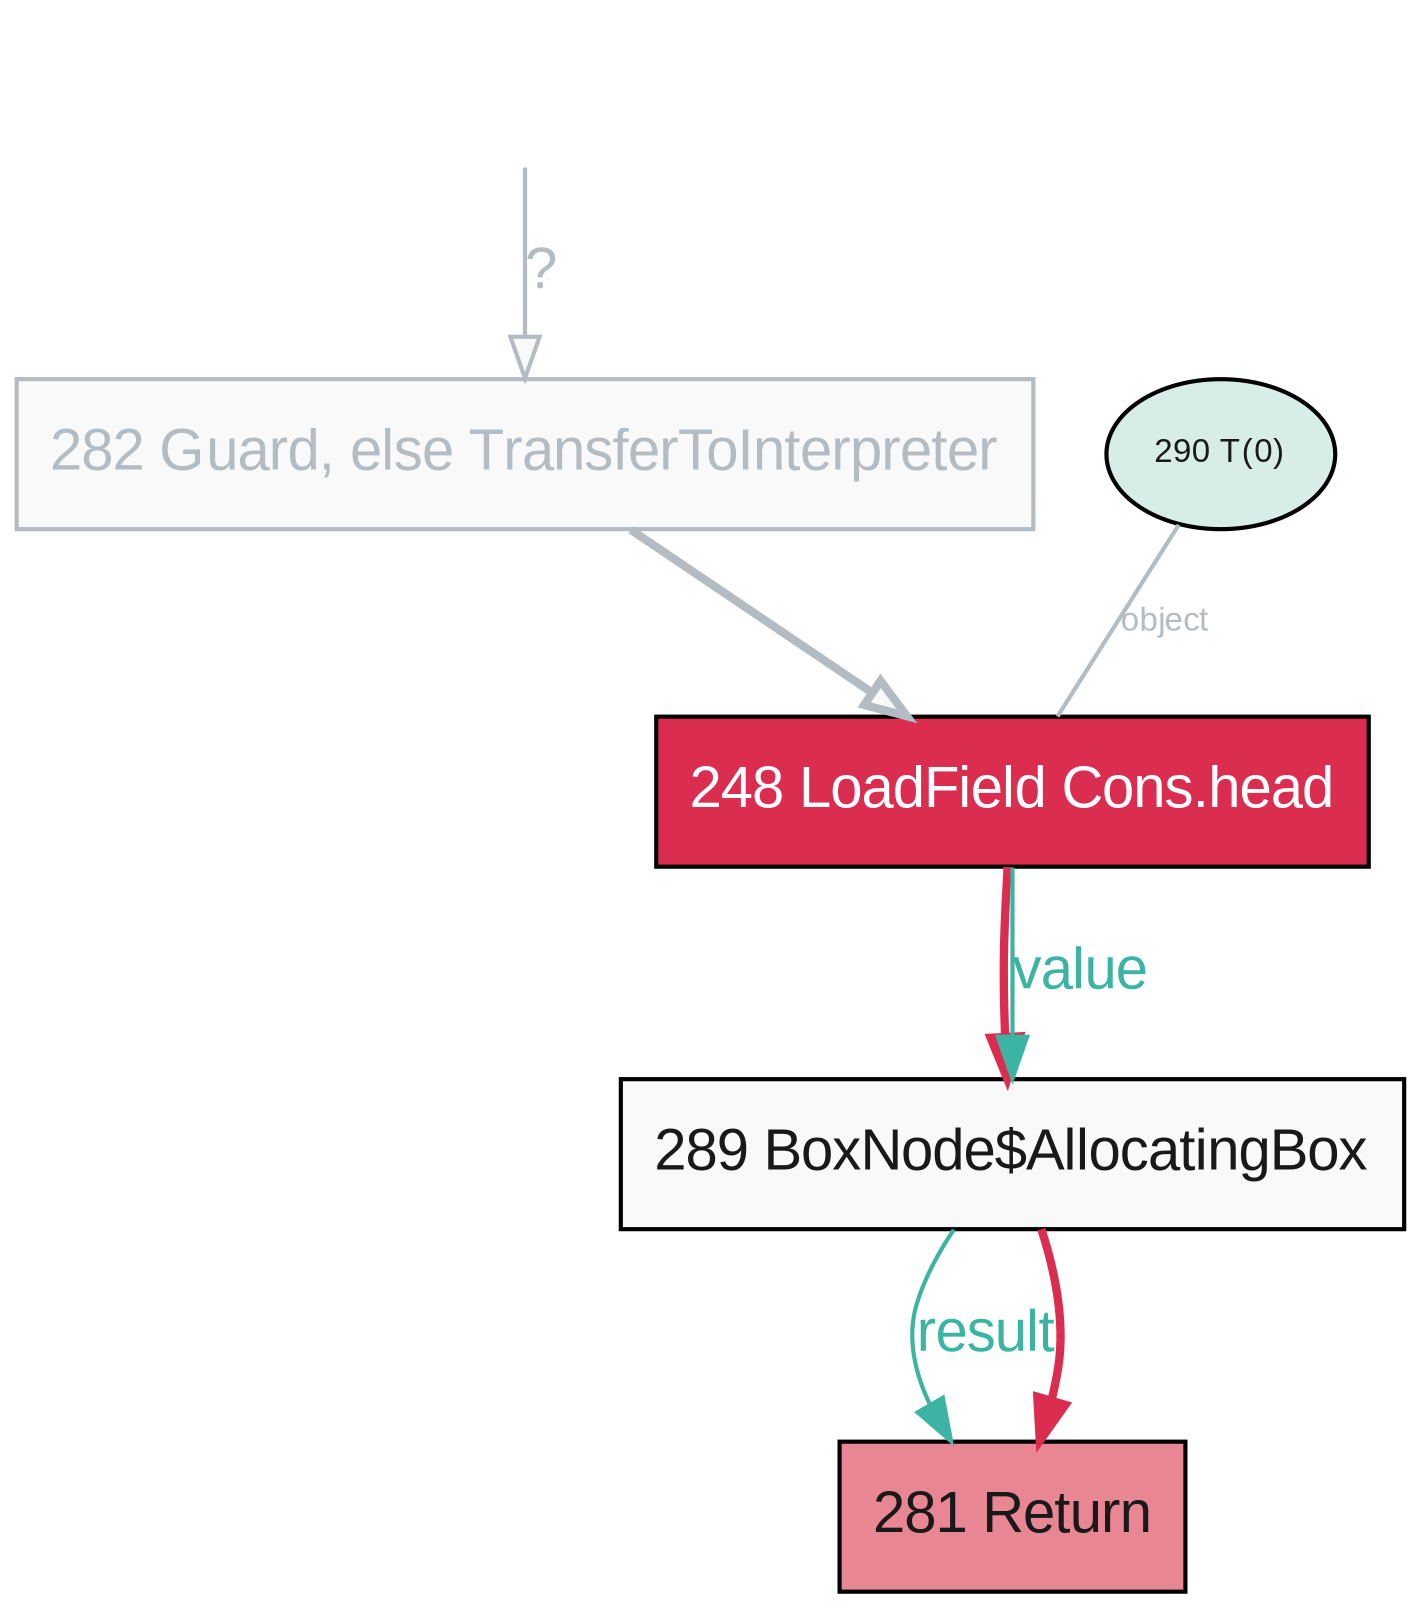
\includegraphics[width=\textwidth]{figures/dot/List.head.specialized.TruffleTier.png}
		\caption{Graal IR of \scalainline{List.head} after field read of \scalainline{head0} is specialized.}
		\label{graalir:cons-head-specialized}
	\end{subfigure}
	\hfill
	\begin{subfigure}[b]{0.4\textwidth}
		\centering
		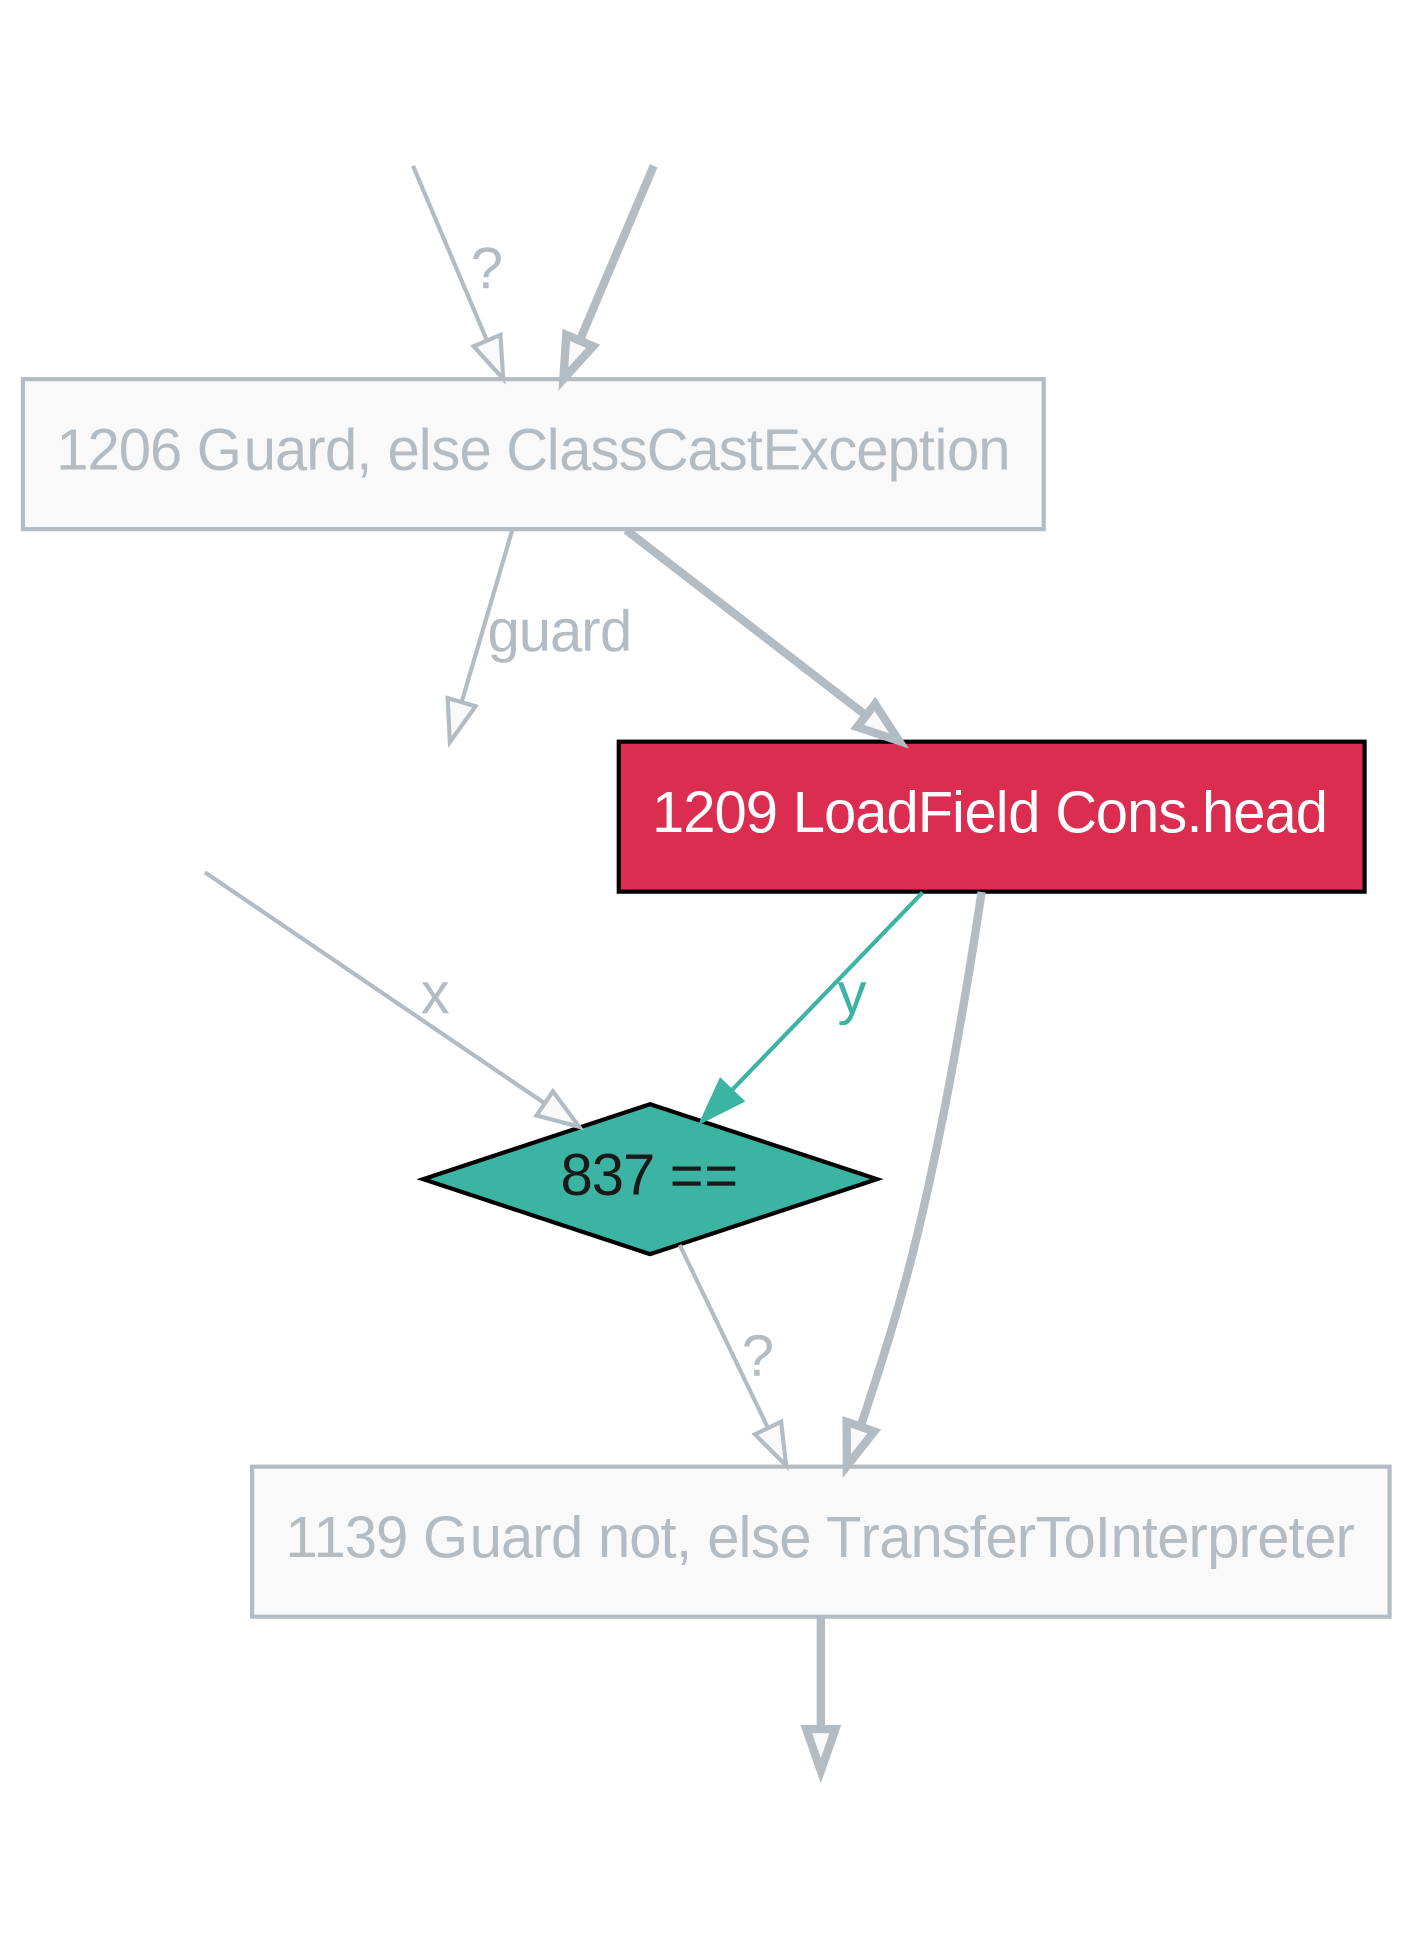
\includegraphics[width=\textwidth]{figures/dot/List.contains.specialized.TruffleTier.png}
		\caption{Graal IR of \scalainline{Cons.head} after being inlined into \scalainline{Cons.contains}}
		\label{graalir:cons-contains-head-focus-specialized}
	\end{subfigure}
	\hfill
\end{figure}

In this section, we will examine previously unboxed code after the specialization of class storage layouts.
Figure \ref{graalir:cons-head-specialized} contains the field access of \scalainline{head0} after the field has been specialized and has the appropriate storage type in the storage layout of \scalainline{Cons[Int]}.
Notice that a box node has been introduced prior to the value of \scalainline{head0} prior to the return node of \scalainline{Cons.head}.
Because the \scalainline{execute} method of a \scalainline{DefDefNode} returns an \javainline{Object}, the return value is preemptively boxed when inspecting the IR of the method.
However, after inlining into the body of \scalainline{Cons.contains}, the box operation is no longer necessary as the boxed value will be immediately unboxed.
Graal will automatically eliminate this type of autoboxing.
When a specialized class instance is used in place of a generic class instance, the field access graph of \scalainline{head0} is the simplest possible graph.

